\documentclass[12pt]{article}

\usepackage[a4paper, left=3cm, right=3cm, top=4cm, bottom=3cm]{geometry}
\usepackage{graphicx}
\usepackage{mathptmx}
\usepackage{setspace}
\usepackage{enumitem}
\usepackage{multirow}
\usepackage{array}
\usepackage{booktabs}
\usepackage{caption}
\usepackage{float}
\usepackage{amsmath}
\usepackage{amssymb}
\usepackage{changepage}
\usepackage[utf8]{inputenc}
\usepackage{natbib}
\usepackage[utf8]{inputenc}   % wajib untuk UTF-8
\usepackage[T1]{fontenc}
\bibliographystyle{agsm}

\usepackage{fancyhdr}
\pagestyle{fancy}
\fancyhf{}
\fancyhead[R]{\thepage}
\renewcommand{\headrulewidth}{0pt}

\renewcommand{\figurename}{Gambar}
\captionsetup[table]{labelsep=period}
\captionsetup[figure]{labelsep=period}

\setstretch{1.5} % atur seluruh dokumen 1,5 spasi
\setlength{\parindent}{0pt}
\setlength{\parskip}{0pt}
\setcounter{page}{5}

\begin{document}

\begin{center}
    \textbf{BAB II}\\
    \textbf{LANDASAN TEORI DAN KERANGKA BERPIKIR}
\end{center}

\textbf{A. Landasan Teori}
\begin{enumerate}
    \item Pendidikan Matematika\\
    \hspace*{1cm}Pentingnya pendidikan matematika didasarkan pada fakta bahwa matematika merupakan aktivitas dasar manusia, sebagaimana halnya musik, seni lukis, sastra, atau bahkan pembuatan sepatu yang berkualitas \citep{hilton1984}. Matematika murni juga membentuk lingkungan tempat aktivitas sehari-hari manusia berlangsung \citep{yig2022}. Menurut Schoenfeld (2000), pendidikan matematika memiliki dua tujuan utama, yaitu tujuan murni dan tujuan terapan. Tujuan matematika murni adalah untuk memahami cara berpikir matematis dan bagaimana mengajarkannya dalam pembelajaran. Sementara itu, tujuan matematika terapan adalah untuk meningkatkan kualitas pengajaran matematika melalui pemahaman yang diperoleh dari matematika murni. Dengan kata lain, matematika merupakan elemen mendasar dalam sains dan teknologi serta penting untuk memahami lingkungan. Oleh karena itu, agar pendidikan matematika berhasil, bidang matematika murni dan terapan harus disajikan secara seimbang \citep{hilton1984}. Karena terdapat hubungan timbal balik antara keduanya, maka tanpa pemahaman mendalam mengenai cara berpikir, belajar, dan mengajar matematika, praktik pembelajaran yang berkelanjutan tidak dapat dikembangkan \citep{schoenfeld2000}.\\
    \hspace*{1cm}Pendidikan matematika merupakan disiplin ilmu di mana berbagai konsep dan topik digunakan secara intensif \citep{turkdogan2015}. Dalam konteks ini, penggunaan konsep-konsep di lapangan serta hubungan antar konsep menjadi komponen penting dalam dinamika bidang tersebut. Dengan pemahaman yang tepat terhadap komponen-komponen ini, pendidikan matematika memberikan perspektif baru bagi para peneliti, sehingga mereka dapat menelaah berbagai topik secara lebih mendalam, mengajukan pertanyaan-pertanyaan baru, dan bahkan menemukan kemungkinan-kemungkinan alternatif (Ernest et al., 2016). Schoenfeld (2000) mengemukakan beberapa pertanyaan yang dieksplorasi dalam pendidikan matematika sebagai berikut:
    \begin{enumerate}
        \item Perspektif teoritis untuk memahami pemikiran, pembelajaran, dan pengajaran;
        \item Berbagai aspek kognisi (misalnya pemikiran matematis, pemahaman siswa, dan kesalahpahaman);
        \item Bukti keberhasilan (situasi di mana siswa dapat belajar memecahkan masalah, induksi, interaksi kelompok, dan penerapan berbagai jenis pengajaran);
        \item Konsekuensi dari berbagai bentuk pengajaran (baik yang bersifat positif maupun negatif).
    \end{enumerate}
    \hspace*{1cm}Dari uraian tersebut dapat disimpulkan bahwa pendidikan matematika memiliki peran yang sangat penting dalam membentuk pola pikir, meningkatkan kualitas pembelajaran, serta mendukung perkembangan ilmu pengetahuan dan teknologi. Keberhasilan pendidikan matematika sangat bergantung pada keseimbangan antara pemahaman konsep secara teoritis dan penerapannya dalam konteks nyata. Dengan pendekatan yang tepat dan pemahaman mendalam terhadap proses berpikir matematis, pembelajaran, serta pengajaran, pendidikan matematika dapat memberikan kontribusi yang signifikan dalam menciptakan pembelajaran yang bermakna dan berkelanjutan.

    \item \textit{Augmented Reality}\\
    \hspace*{1cm}\textit{Augmented reality} memungkinkan objek virtual yang dihasilkan oleh komputer ditempatkan di atas objek fisik secara \textit{real-time} \citep{ozdemir2018}. Penggabungan antara dunia nyata dan dunia maya membuat batas di antara keduanya menjadi sangat tipis. \textit{Augmented reality} merupakan sebuah sistem yang memiliki tiga karakteristik utama, yaitu: (1) menggabungkan dunia nyata dan dunia virtual; (2) interaktif secara \textit{real-time}; dan (3) mampu menyajikan tampilan tiga dimensi \citep{azuma1997}. Teknologi \textit{augmented reality} dapat memuat video, suara, gambar, teks, dan model \textit{3D} \citep{tekedere2016}. Pengguna dapat berinteraksi dengan objek virtual yang dimasukkan ke dalam lingkungan sekitarnya dan memperoleh pengalaman dalam berinteraksi dengan komputer \citep{cai2014}. Penggunaan teknologi \textit{augmented reality} dalam pembelajaran memungkinkan siswa untuk menjelajahi dunia secara interaktif dan kolaboratif \citep{antonioli2014}. Multimedia interaktif berbasis \textit{augmented reality} menyediakan fasilitas bagi pengguna untuk berinteraksi dengan objek \textit{3D}, yang membantu siswa dalam memahami konsep-konsep tertentu dengan lebih mudah \citep{martin2010}.\\
    \hspace*{1cm}Penggunaan teknologi \textit{augmented reality} berkontribusi terhadap perkembangan siswa, baik dalam aspek afektif maupun kognitif, serta menjadikan pembelajaran sebagai proses yang lebih efisien dan menarik \citep{tomi2013}. Pembelajaran dengan aplikasi \textit{augmented reality} berbasis seluler juga efektif digunakan dalam kegiatan tatap muka \citep{lin2013}. Selain keunggulan tersebut, \textit{augmented reality} memberikan kontribusi positif dalam proses belajar dengan meningkatkan pemahaman, persepsi konsep, dan membantu siswa berpikir secara terstruktur, terutama pada mata pelajaran seperti astronomi, sains, dan matematika \citep{bujak2013}.\\
    \hspace*{1cm}Berdasarkan uraian di atas, dapat disimpulkan bahwa teknologi \textit{augmented reality} memiliki potensi besar dalam mendukung pengembangan kemampuan spasial siswa. Dengan karakteristiknya yang menggabungkan dunia nyata dan virtual secara interaktif dan \textit{real-time}, \textit{augmented reality} mampu menyajikan pengalaman belajar yang imersif melalui tampilan tiga dimensi. Teknologi ini tidak hanya memperkaya aspek kognitif dan afektif siswa, tetapi juga mempermudah pemahaman konsep-konsep abstrak melalui visualisasi yang konkret. Oleh karena itu, integrasi \textit{augmented reality} dalam pembelajaran, khususnya dalam bidang sains dan matematika, dapat menjadi alternatif inovatif yang meningkatkan efektivitas, keterlibatan, dan pemahaman siswa secara menyeluruh.

    % PERBAIKI MAIER
    \item Kemampuan Spasial dan Teknologi\\
    \hspace*{1cm}Banyak istilah berbeda digunakan dalam literatur untuk mendefinisikan dan menggambarkan kemampuan spasial \citep{ozcakir2021augmented}. Beberapa istilah tersebut antara lain pemikiran spasial \citep{yakimanskaya1991}, pengertian spasial \citep{nctm1989}, keterampilan spasial \citep{tartre1990}, dan penalaran spasial \citep{battista2007}. Istilah-istilah ini digunakan oleh para peneliti untuk menjelaskan proses visualisasi mental, manipulasi, serta rotasi terhadap angka dan bentuk. Secara umum, inti dari definisi kemampuan spasial mengacu pada ide-ide seperti kemampuan untuk memutar, mengubah, atau membayangkan suatu objek serta memanipulasi sifat-sifatnya secara mental \citep{ozcakir2021augmented}. Dengan kata lain, kemampuan spasial merupakan keterampilan dalam membayangkan bentuk-bentuk geometri dan bagaimana bentuk tersebut berubah ketika diputar atau dimanipulasi dalam pikiran.\\
    \hspace*{1cm}Selain istilah yang bervariasi, terdapat pula beragam klasifikasi komponen kemampuan spasial yang diajukan oleh para peneliti. \citet{battista1994} membagi kemampuan spasial menjadi dua komponen, yaitu orientasi spasial dan visualisasi spasial. Sementara itu, \citet{pellegrino1982} mengkategorikan menjadi hubungan spasial dan visualisasi spasial. \citet{linn1985} bahkan membagi kemampuan spasial menjadi tiga elemen, yakni perputaran mental, persepsi spasial, dan visualisasi spasial. Meskipun terdapat perbedaan dalam pengkategorian, semua komponen tersebut dapat dipahami secara logis dan relevan dengan kemampuan berpikir spasial manusia \citep{ozcakir2021augmented}. Berangkat dari perkembangan teknologi dan kompleksitas tantangan visual-spasial saat ini, Maier (1996) menyatakan bahwa klasifikasi tersebut perlu diperluas. Maier (1996) mengusulkan lima elemen kemampuan spasial, yaitu perputaran mental, persepsi spasial, visualisasi spasial, hubungan spasial, dan orientasi spasial. Ia menekankan bahwa kemajuan teknologi menuntut pelatihan menyeluruh terhadap kelima elemen ini untuk mendukung perkembangan keterampilan spasial yang lebih mendalam.\\
    \hspace*{1cm}Kemampuan spasial merupakan aspek penting dalam proses kognitif yang melibatkan kemampuan untuk memvisualisasikan, memanipulasi, dan merotasi objek secara mental. Berbagai istilah telah digunakan dalam literatur untuk menggambarkan kemampuan ini, seperti pemikiran spasial, pengertian spasial, keterampilan spasial, dan penalaran spasial, yang semuanya mengarah pada proses visualisasi dan manipulasi bentuk atau angka dalam pikiran. Para peneliti juga mengelompokkan komponen kemampuan spasial dalam beberapa kategori, mulai dari dua hingga lima elemen utama, antara lain visualisasi spasial, orientasi spasial, hubungan spasial, persepsi spasial, dan perputaran mental. Meskipun terdapat perbedaan dalam klasifikasi tersebut, seluruh elemen tersebut dianggap relevan dan saling melengkapi. Seiring dengan perkembangan teknologi, pelatihan terhadap seluruh komponen kemampuan spasial menjadi semakin penting, khususnya dalam bidang pendidikan dan pembelajaran, guna meningkatkan efektivitas pemahaman konsep-konsep abstrak yang membutuhkan representasi visual.

    \item Bangun Ruang Sisi Datar\\
    \hspace*{1cm}Berdasarkan Permendikbud Nomor 37 Tahun 2018 tentang Kompetensi Inti dan Kompetensi Dasar, materi Matematika SMP Kelas VIII Semester Genap mencakup pembahasan tentang bangun ruang sisi datar. Penelitian ini difokuskan pada materi tersebut, dengan kompetensi dasar yang ditampilkan pada Tabel \ref{kikd} berikut:
    \begin{table}[H]
        \centering
        \caption{KI dan KD Materi Bangun Ruang Sisi Datar}
        \label{kikd}
        \begin{tabular}{|p{7cm}|p{7cm}|}
            \hline
            \textbf{Kompetensi Inti 3 (Pengetahuan)} & \textbf{Kompetensi Inti 4 (Keterampilan)} \\
            \hline
            Memahami dan menerapkan pengetahuan (faktual, konseptual, dan prosedural) berdasarkan rasa ingin tahunya tentang ilmu pengetahuan, teknologi, seni, budaya terkait fenomena dan kejadian tampak mata. &
            Mengolah, menyaji dan menalar dalam ranah konkret (menggunakan, mengurai, merangkai, memodifikasi, dan membuat) dan ranah abstrak (menulis, membaca, menghitung, menggambar, dan mengarang) sesuai dengan yang dipelajari di sekolah dan sumber lain yang sama dalam sudut pandang/teori. \\
            \hline
            \textbf{Kompetensi Dasar 3.9} & \textbf{Kompetensi Dasar 4.9}\\
            \hline
            Membedakan dan menentukan luas permukaan dan volume bangun ruang sisi datar (kubus, balok, prisma, limas). & Menyelesaikan masalah yang berkaitan dengan luas permukaan dan volume bangun ruang sisi datar (kubus, balok, prisma, dan limas), serta gabungannya.\\
            \hline
        \end{tabular}
    \end{table}
    \hspace*{1cm}Jenis bangun ruang sisi datar yang dibahas dalam materi SMP meliputi kubus, balok, prisma, dan limas. Pembahasan difokuskan pada volume dan luas permukaan bangun ruang tersebut.
    \begin{enumerate}
        \item Luas Permukaan\\
        \hspace*{1cm}Luas permukaan adalah jumlah luas seluruh sisi suatu bangun ruang. Sebagai contoh, pada kubus, luas permukaan merupakan jumlah luas dari keenam sisinya. Karena kubus memiliki enam sisi yang kongruen (sama besar), maka luas permukaan kubus dapat dihitung dengan mengalikan luas satu sisi dengan enam. Penjelasan lebih lanjut dapat dilihat pada Gambar \ref{kubusjaring}.
        \begin{figure}[H]
            \centering
            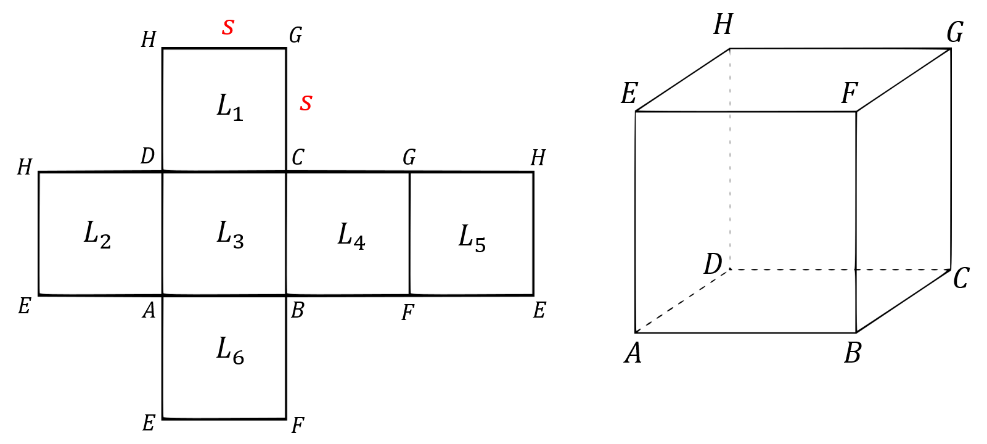
\includegraphics[width=0.6\textwidth]{images/kubusdanjaring.png}
            \caption{Kubus dan Jaring-jaringnya}
            \label{kubusjaring}
        \end{figure}
        \hspace*{1cm}Pada Gambar \ref{kubusjaring}, disajikan kubus dengan enam buah sisi sama besar.\\
        \( L_1 = L_2 = L_3 = L_4 = L_5 = L_6 \)

        Sehingga seluruh luas permukaan kubus adalah\\
        $ L = L_1 + L_2 + L_3 + L_4 + L_5 + L_6 $\\
        $ L = 6 \times L_1 $\\
        $ L = 6 \times s \times s = 6 \times s^2 .$\\
        Cara mencari luas permukaan balok sedikit berbeda dengan kubus karena ukuran sisi-sisinya tidak semuanya sama. Perbedaan ini ditunjukkan pada Gambar \ref{balokjaring}.
        \begin{figure}[H]
            \centering
            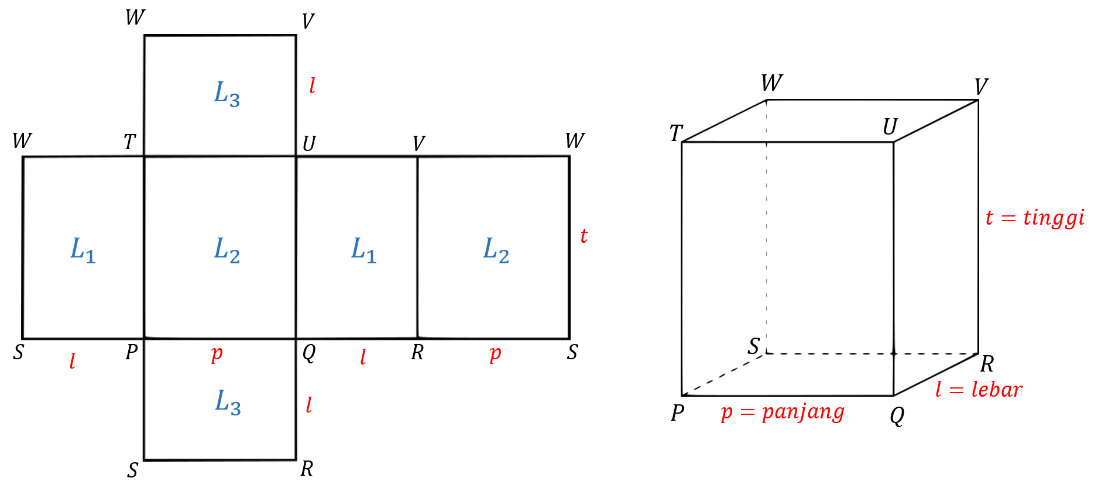
\includegraphics[width=0.6\textwidth]{images/balokdanjaring.png}
            \caption{Balok dan Jaring-jaringnya}
            \label{balokjaring}
        \end{figure}
        \hspace*{1cm}Pada bangun balok, sisi-sisi yang berhadapan memiliki ukuran yang sama. Misalnya, sisi depan sama dengan sisi belakang, sisi kiri sama dengan sisi kanan, serta sisi atas sama dengan sisi bawah. Pada Gambar 2, masing-masing sisi diberi label untuk mempermudah pemahaman. Luas permukaan balok dirumuskan sebagai berikut:\\
        $ L = 2 \times L_1 + 2 \times L_2 + 2 \times L_3 $\\
        $ L = 2 \times l \times t + 2 \times p \times t + 2 \times l \times p $\\
        $ L = 2 \times (l \times t + p \times t + l \times p) $\\
        Keterangan:\\
        $ L = \text{Luas Permukaan} $\\
        $ p = \text{Panjang} $\\
        $ l = \text{Lebar} $\\
        $ t = \text{Tinggi} $\\
        Berikut ini merupakan contoh soal untuk menghitung luas permukaan kubus dan balok:
        \begin{enumerate}[label=\arabic*)]
            \item Sebuah balok memiliki luas permukaan \( 236 \text{~cm}^2 \). Jika lebar dan tinggi balok masing-masing 8 dan 6 cm, tentukanlah panjang balok tersebut.\\
            Pembahasan:\\
            $ L = 2 \times (l \times t + p \times t + l \times p) $\\
            $ L = 2 \times (8 \times 6 + p \times 6 + 8 \times p) $\\
            $ L = 2 \times (48+6p+8p)$\\
            $ L = 2 \times (48+14p)$\\
            $ 236 = 96 + 28p $\\
            $ 28p = 236 - 96 = 140 $\\
            $ p = \frac{140}{28} = 5$\\
            Jadi panjang balok tersebut adalah 5 cm.
            \item Diketahui sebuah kubus memiliki panjang rusuk 12 cm. Maka luas permukaan kubus tersebut adalah \dots \\
            Pembahasan:\\
            $ L = 6 \times s^2 $\\
            $ L = 6 \times 12^2$\\
            $ L = 6 \times 144 = 684$\\
            Jadi luas permukaan kubus tersebut adalah \( 684 \text{ cm}^2 \).
        \end{enumerate}
        \hspace*{1cm}Kubus dan balok memiliki semua sisi berbentuk segiempat. Pada kubus, seluruh sisinya berbentuk persegi, sedangkan pada balok terdapat sisi-sisi yang berbentuk persegi panjang. Lalu, bagaimana jika suatu bangun ruang memiliki bentuk sisi yang lebih kompleks, seperti yang ditunjukkan pada Gambar \ref{jenisprisma} berikut?
        \begin{figure}[H]
            \centering
            
\includegraphics[width=0.6\textwidth]{images/jenisprisma.png}
            \caption{Jenis-jenis Prisma}
            \label{jenisprisma}
        \end{figure}
        \hspace*{1cm}Bangun pada Gambar \ref{jenisprisma} disebut sebagai prisma. Prisma memiliki alas dan tutup yang kongruen (sama bentuk dan ukuran), serta dihubungkan oleh sisi-sisi tegak berbentuk segiempat. Luas permukaan prisma dapat dihitung dengan menjumlahkan luas alas dan tutup, serta luas seluruh sisi tegaknya. Luas permukaan prisma sama dengan luas jaring-jaringnya. Berikut disajikan contoh perhitungan luas permukaan sebuah prisma.
        \begin{enumerate}[label=\arabic*)]
            \item Diketahui sebuah prisma dengan alas berbentuk segitiga siku-siku. Sudut siku-siku terletak di \( \angle ACB \). Jika tinggi prisma adalah 8 cm, maka luas permukaan prisma tersebut adalah \dots\\
            \begin{figure}[H]
                \centering
                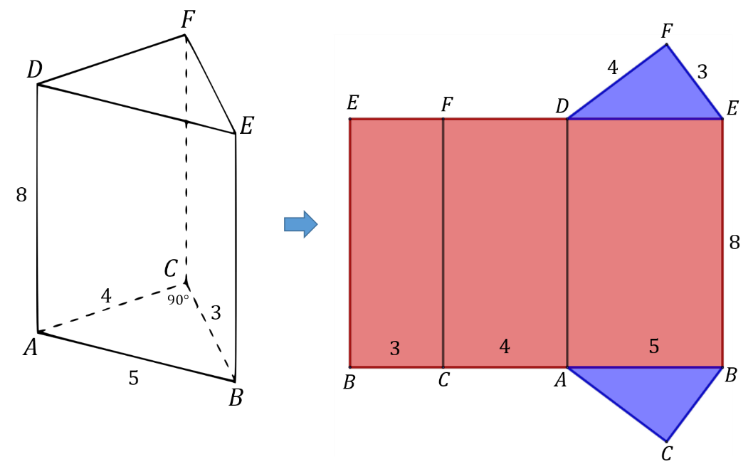
\includegraphics[width=0.6\textwidth]{images/prismasegitigasiku.png}
                \caption{Prisma Segitiga Siku-siku}
                \label{prismasegitigasiku}
            \end{figure}
            Pembahasan:\\
            Luas permukaan prisma dapat dicari dengan terlebih dahulu menentukan luas alas prisma, yang pada Gambar~\ref{prismasegitigasiku} diberi warna biru. Jika alas prisma berbentuk segitiga, maka rumus luas alasnya adalah:\\
            $ L_a = \frac{1}{2} \times a \times t $\\
            $ L_a = \frac{1}{2} \times BC \times AC$\\
            $ L_a = \frac{1}{2} \times 3 \times 4 = 6$\\
            dimana \(a\) adalah panjang alas segitiga, dan \(t\) adalah tinggi segitiga. Untuk selanjutnya bisa dicari luas sisi-sisi tegaknya dengan cara\\
            $ L_t = (BC + CA + AB) \times BE = \text{keliling alas} \times \text{tinggi prisma} $\\
            $ L_t = (3+4+5) \times 8 = 96 $\\
            sehingga didapat luas permukaan prisma\\
            $ L = 2\times L_a + L_t = 2 \times 6 + 96 = 108. $\\
            Jadi luas permukaan prisma tersebut adalah 108 \( \text{cm}^2.\)
        \end{enumerate}
        \hspace*{1cm}Sebelumnya telah dipelajari cara menghitung luas permukaan bangun ruang sisi datar yang memiliki bentuk alas dan tutup yang sama, seperti kubus, balok, dan prisma. Sekarang, bagaimana jika bangun ruang yang akan dicari luas permukaannya memiliki bentuk seperti yang ditunjukkan pada Gambar \ref{jenislimas} berikut?
        \begin{figure}[H]
            \centering
            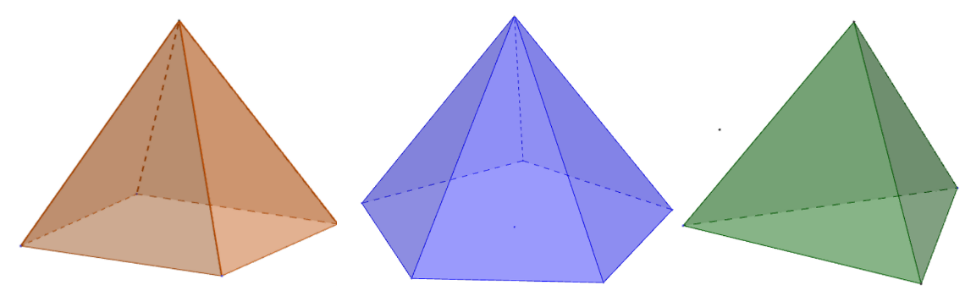
\includegraphics[width=0.6\textwidth]{images/jenislimas.png}
            \caption{Jenis-jenis Limas}
            \label{jenislimas}
        \end{figure}
        \hspace*{1cm}Bangun seperti yang ditunjukkan pada Gambar~\ref{jenislimas} disebut limas. Limas memiliki alas berbentuk bangun datar dan mengerucut ke atas menyerupai piramida. Untuk menghitung luas permukaan limas, terlebih dahulu disajikan jaring-jaring limas segiempat pada Gambar~\ref{limasdanjaring}.
        \begin{figure}[H]
            \centering
            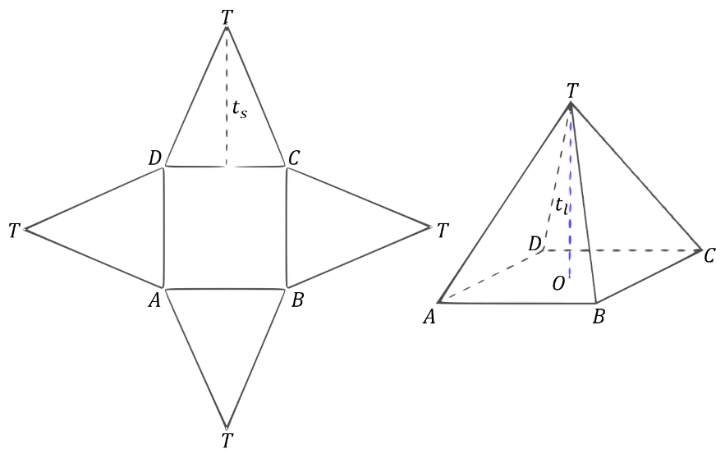
\includegraphics[width=0.6\textwidth]{images/limasdanjaringnya.png}
            \caption{Limas dan Jaring-jaringnya}
            \label{limasdanjaring}
        \end{figure}
        Keterangan:\\
        $ t_s = \text{tinggi sisi tegak} $\\
        $ t_l = \text{tinggi limas} $\\
        $ ABCD = \text{alas limas} $\\
        $ CDT,BCT,ABT,ADT = \text{sisi tegak} $\\
        \hspace*{1cm}Pada limas segiempat seperti yang ditunjukkan pada Gambar~\ref{limasdanjaring}, terdapat empat buah sisi tegak yang memiliki bentuk yang sama, serta satu alas limas yang berbentuk persegi, yaitu alas ABCDABCD. Dengan demikian, luas permukaan limas segiempat dapat dihitung dengan menjumlahkan luas alas dan empat kali luas salah satu sisi tegaknya.
        \begin{equation}
            L_p = 4 \times L_s + L_a
        \end{equation}
        Keterangan:\\
        $ L_p = \text{luas permukaan} $\\
        $ L_s = \text{luas sisi tegak} $\\
        $ L_a = \text{luas alas} $\\
        Diberikan contoh mencari luas permukaan limas seperti berikut.\\
        \begin{enumerate}[label=\arabic*)]
            \item Diketahui limas \( T.ABCD \) dengan alas berbentuk persegi. Jika panjang \( AB = 4\text{ cm} \), dan tinggi sisi tegak limas adalah 5 cm, maka luas permukaan limas tersebut adalah \dots\\
            Pembahasan:\\
            $ L_p = 4 \times L_s + L_a $\\
            $ L_p = 4 \times \frac{1}{2} \times 4 \times 5 + 4 \times 4 $\\
            $ L_p = 40 + 16 = 56 $\\
            Jadi luas permukaan limas tersebut adalah \( 56 \text{ cm}^2 \).\\
        \end{enumerate}

    \end{enumerate}

\end{enumerate}

\textbf{B. Kajian Penelitian yang Relevan}\\
\hspace*{1cm}Berikut ini adalah beberapa penelitian yang relevan dengan pengembangan media pembelajaran interaktif berbasis Augmented Reality pada materi bangun ruang sisi datar, antara lain:
\begin{enumerate}
    \item Penelitian yang dilakukan oleh \citet{maulana2020} dengan judul \textit{“The Use of Mobile-Based Augmented Reality in Science Learning to Improve Learning Motivation”} bertujuan untuk mengkaji pengaruh penggunaan media berbasis \textit{augmented reality} pada perangkat \textit{Android} terhadap peningkatan motivasi belajar siswa. Penelitian ini menggunakan metode \textit{quasi-experimental} dengan desain \textit{pretest-posttest control group}. Berdasarkan hasil uji statistik menggunakan \textit{SPSS}, diperoleh nilai signifikansi sebesar 0{,}002 yang lebih kecil dari 0{,}025. Hal ini menunjukkan adanya perbedaan skor rata-rata antara kelas kontrol dan kelas eksperimen. Dengan demikian, dapat disimpulkan bahwa pembelajaran menggunakan media \textit{augmented reality} berbasis \textit{Android} berpengaruh positif terhadap proses pembelajaran di kelas, yang ditunjukkan dengan meningkatnya motivasi belajar siswa.
    Persamaan antara penelitian ini dengan penelitian yang sedang dilakukan terletak pada penggunaan media pembelajaran berbasis \textit{augmented reality} pada perangkat \textit{Android}. Adapun perbedaannya terletak pada tujuan penelitian, di mana penelitian ini bertujuan untuk mengembangkan media pembelajaran interaktif berbasis \textit{augmented reality}.
    \item Penelitian yang dilakukan oleh \citet{suprapto2021} dengan judul \textit{“The Use of Physics Pocketbook Based on Augmented Reality on Planetary Motion to Improve Student’s Learning Achievement”}. Penelitian ini bertujuan untuk mengembangkan buku saku berbasis \textit{augmented reality} pada materi gerak planet, fokus pengembangan terletak pada peningkatan prestasi belajar siswa. Penelitian ini menggunakan model \textit{ADDIE} (\textit{Analysis, Design, Development, Implementation,} dan \textit{Evaluation}). Uji coba dilakukan kepada 30 siswa yang terdiri dari 17 perempuan dan 13 laki-laki berusia 16–17 tahun, bertempat di sekolah menengah umum di Surabaya. Parameter evaluasi meliputi kualitas buku saku berbasis \textit{AR}, prestasi belajar siswa, dan luaran penelitian. Teknik analisis data menggunakan statistik deskriptif, \textit{N-gain score}, dan \textit{independent t-test}. Hasil penelitian menunjukkan bahwa: 1) proses pengembangan buku saku berbasis \textit{AR} pada pergerakan planet memenuhi kriteria kualitas produk valid, praktis, dan efektif; 2) prestasi belajar siswa meningkat dilihat dari hasil nilai \textit{pretest-posttest} dengan rata-rata skor \textit{gain} adalah 0{,}63 berkategori sedang, di mana siswa laki-laki berkinerja lebih baik dari siswa perempuan; 3) melalui pengembangan buku saku berbasis \textit{AR}, dihasilkan beberapa artikel di jurnal dan media buku saku berbasis \textit{AR}. Sehingga, rekomendasi dari penelitian ini adalah menggunakan \textit{AR} sebagai media pembelajaran dalam konsep fisika abstrak lainnya. Persamaan dengan penelitian sebelumnya adalah keduanya merupakan penelitian pengembangan media pembelajaran berbasis \textit{augmented reality}. Sedangkan perbedaannya terletak pada materi yang disampaikan, model penelitian, dan bentuk media.
    \item Penelitian yang dilakukan oleh \citet{derlina2020blended} dengan judul \textit{“Blended Learning in English and English-medium Physics Classes Using Augmented Reality, Edmodo, and Tinkercad Media”}. Penelitian ini bertujuan untuk mengetahui efektivitas \textit{blended learning} untuk meningkatkan hasil belajar siswa dalam bahasa Inggris dan fisika dengan menggunakan \textit{AR}, \textit{Edmodo}, dan \textit{TinkerCad}. Ini merupakan penelitian \textit{quasi experiment} dengan data yang diperoleh secara acak dari 70 siswa di SMA 2 Lubuk Pakam, Indonesia. Sampel dibagi menjadi dua kelompok, yang pertama kelas eksperimen yang menerapkan pembelajaran \textit{blended}, dan kedua kelas kontrol yang menerapkan pembelajaran konvensional. Instrumen penelitian berupa tes hasil belajar, berupa tes objektif yang diberikan pada saat \textit{pretest} dan \textit{post-test} dalam bentuk lembar observasi. Efektivitas pembelajaran \textit{blended} dalam meningkatkan hasil belajar siswa dianalisis menggunakan \textit{independent sample t-test} dengan \textit{SPSS 17}. Hasil penelitian menunjukkan bahwa pembelajaran \textit{blended} secara efektif meningkatkan hasil belajar siswa dilihat dari hasil uji \textit{t-test} sampel mandiri dan berpasangan masing-masing sebesar 0{,}148 dan 0{,}000. Dari penelitian ini dapat disimpulkan bahwa pembelajaran \textit{blended} menggunakan \textit{AR}, \textit{Edmodo}, dan \textit{TinkerCad} secara efektif meningkatkan hasil belajar siswa dan membuat siswa menjadi aktif. Perbedaan dengan penelitian sebelumnya adalah, penelitian Derlina dan tim menggunakan tambahan media yaitu \textit{Edmodo} serta dilakukan secara \textit{blended}. Sedangkan persamaannya adalah penggunaan \textit{TinkerCad} untuk membuat objek tiga dimensi.
\end{enumerate}

\textbf{C. Kerangka Berpikir}\\
\hspace*{1cm}Kerangka berpikir dalam penelitian dan pengembangan ini dilatarbelakangi oleh permasalahan yang ditemukan di SMP Negeri 3 Kalikajar, yaitu bahan ajar yang digunakan oleh pendidik masih terbatas pada buku teks dan LKS. Selain itu, peserta didik masih mengalami kesulitan dalam menyelesaikan soal-soal yang berkaitan dengan bangun ruang. Berdasarkan permasalahan tersebut, peneliti menawarkan solusi dengan mengembangkan produk berupa media pembelajaran berbasis Augmented Reality. Diharapkan, media pembelajaran berbasis AR ini dapat mempermudah peserta didik dalam memahami materi bangun ruang serta meningkatkan motivasi mereka dalam belajar.\\
\hspace*{1cm}Augmented Reality adalah teknologi yang mampu menampilkan objek 3D seolah-olah terlihat nyata dan menyatu dengan lingkungan sekitar. Teknologi ini sesuai untuk digunakan dalam materi Bangun Ruang Sisi Datar, di mana objek bangun ruang sering kali perlu divisualisasikan secara lebih konkret. Hal ini disebabkan oleh keterbatasan gambar 2D dalam menunjukkan bentuk secara menyeluruh, sehingga dengan Augmented Reality, peserta didik dapat melihat bentuk bangun ruang secara lebih nyata dan mendalam. Proses perancangan media pembelajaran diawali dengan wawancara bersama pendidik mata pelajaran matematika. Dari hasil wawancara diperoleh informasi bahwa peserta didik mengalami kesulitan saat mengerjakan soal yang berkaitan dengan bangun ruang 3D, terutama dalam mengidentifikasi bentuk bangun prisma dan limas.\\
\hspace*{1cm}Proses selanjutnya adalah mempelajari materi bangun ruang dan mengidentifikasi bagian materi yang perlu divisualisasikan ke dalam bentuk Augmented Reality (AR). Setelah materi teridentifikasi, model bangun ruang 3D akan dibuat menggunakan aplikasi Blender. Selanjutnya, materi pembelajaran yang terintegrasi dengan AR dikembangkan dalam bentuk website yang dapat diakses melalui ponsel peserta didik. Media pembelajaran yang telah dikembangkan akan divalidasi oleh ahli, kemudian direvisi sesuai dengan masukan yang diberikan sebelum digunakan dalam proses pembelajaran. Setelah validasi, media akan diuji coba terlebih dahulu pada kelas kecil. Jika masih ditemukan kekurangan, akan dilakukan perbaikan sebelum diujicobakan pada kelas besar. Pada tahap uji coba kelas, peneliti akan mengumpulkan data berupa respons peserta didik terhadap media pembelajaran yang dikembangkan. Alur kerangka berpikir dalam penelitian ini dapat dilihat pada Gambar IV berikut.

\newpage
\begin{center}
    \textbf{BAB III}\\
    \textbf{METODE PENELITIAN}
\end{center}

\textbf{A. Model Pengembangan}

\hspace*{1cm}Penelitian ini termasuk dalam jenis penelitian pengembangan atau \textit{Research and Development} (R\&D). Menurut \citet{sugiyono2015}, model pengembangan atau \textit{Research and Development} merupakan metode penelitian yang bertujuan untuk menciptakan produk tertentu berdasarkan analisis kebutuhan dan melalui tahapan pengujian produk. Produk yang dikembangkan dalam penelitian ini adalah media pembelajaran berbasis \textit{Augmented Reality} pada materi bangun ruang sisi datar. Model pengembangan yang digunakan dalam penelitian ini adalah model ADDIE (\textit{Analysis}, \textit{Design}, \textit{Development}, \textit{Implementation}, and \textit{Evaluation}).

% LENGKAPI REFERENCE CAHYADI
\hspace*{1cm}Model ADDIE merupakan salah satu model desain pembelajaran yang menggambarkan langkah-langkah dasar dalam sistem pembelajaran yang mudah diterapkan \citep{cahyadi2019}. Model ini dipilih karena disusun secara sistematis dan terstruktur untuk memecahkan permasalahan pembelajaran sesuai dengan kebutuhan serta karakteristik peserta didik. Model ADDIE terdiri dari lima tahap, yaitu: (1) analisis, (2) perancangan, (3) pengembangan, (4) implementasi, dan (5) evaluasi.\\


\textbf{B. Prosedur Pengembangan}

\hspace*{1cm}Model ADDIE memiliki beberapa tahapan prosedur pengembangan yang ditunjukkan pada Gambar~\ref{gambar-addie} berikut.
\begin{figure}[H]
  \centering
  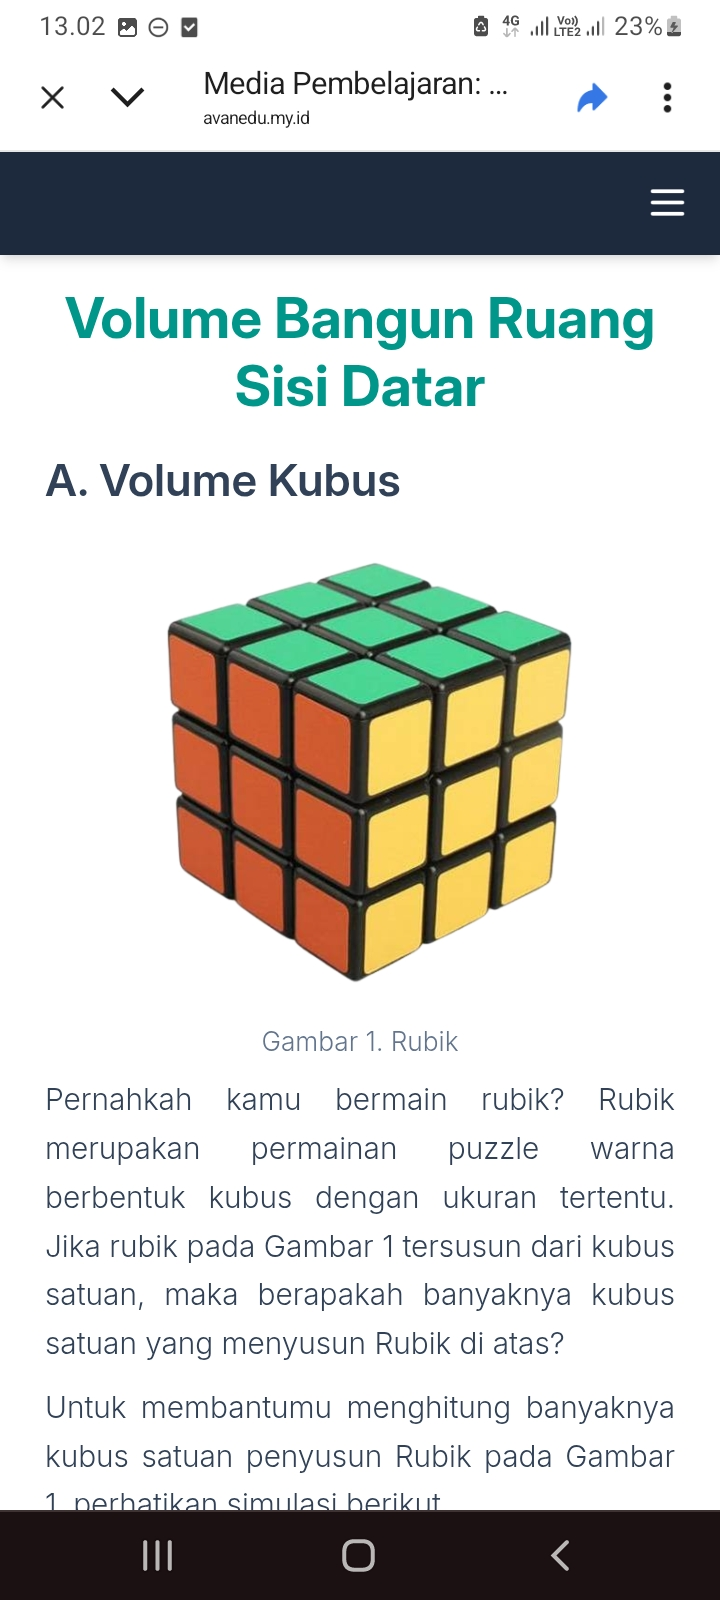
\includegraphics[width=0.2\textwidth]{images/materi1.jpg}
  \caption{Tahapan prosedur pengembangan model ADDIE}
  \label{gambar-addie}
\end{figure}

\hspace*{1cm}Menurut Mulyatiningsih (dalam Setyadi \& Saefudin, 2019), model ADDIE merupakan akronim dari Analysis, Design, Development, Implementation, dan Evaluation. Berikut penjelasan dari masing-masing tahapan.
\begin{enumerate}
    \item Analisis \textit{(Analysis)}\\
    \hspace*{1cm}Pada tahap analisis, peneliti melakukan analisis terhadap tiga hal, yaitu: analisis kebutuhan, analisis kurikulum, dan analisis karakteristik peserta didik.
    \begin{enumerate}
        \item Analisis Kebutuhan\\
        \hspace*{1cm}Pada tahap analisis kebutuhan, peneliti mengidentifikasi permasalahan yang menjadi dasar pengembangan media pembelajaran berbasis Augmented Reality. Permasalahan yang dianalisis antara lain mencakup materi yang dianggap sulit oleh peserta didik serta kebutuhan akan sumber belajar yang sudah tersedia di sekolah namun belum dimanfaatkan secara maksimal.
        \item Analisis Kurikulum\\
        \hspace*{1cm}Pada tahap analisis kurikulum, peneliti mengkaji kurikulum yang digunakan di SMP Negeri 3 Kalikajar serta Kompetensi Dasar yang harus dicapai oleh peserta didik, guna menentukan materi pembelajaran yang relevan untuk dikembangkan.
        \item Analisis karakteristik Peserta Didik\\
        \hspace*{1cm}Pada tahap analisis karakteristik peserta didik, peneliti melakukan observasi terhadap proses pembelajaran melalui wawancara langsung dengan pendidik kelas VIII SMP Negeri 3 Kalikajar. Selain itu, observasi mengenai karakteristik peserta didik juga dilakukan melalui penyebaran angket pra-penelitian menggunakan Google Form kepada peserta didik.
    \end{enumerate}
    \item Perancangan \textit{(Design)}\\
    \hspace*{1cm}Pada tahap perancangan, peneliti merancang media pembelajaran berbasis \textit{Augmented Reality}, mengumpulkan berbagai referensi, serta menyusun instrumen penelitian yang dikembangkan berdasarkan hasil analisis sebelumnya. Instrumen tersebut mencakup aspek kelayakan isi, tampilan, bahasa, serta kesesuaian materi dengan teknologi \textit{Augmented Reality}. Setelah itu, media dikonsultasikan kepada dosen pembimbing, sedangkan instrumen penilaian divalidasi oleh dosen ahli untuk memperoleh instrumen yang layak dan valid.
    \item Pengembangan \textit{(Development)}\\
    \hspace*{1cm}Pada tahap pengembangan, peneliti merealisasikan pembuatan media pembelajaran berbasis \textit{Augmented Reality}. Adapun hal-hal yang dilakukan peneliti pada tahap ini adalah sebagai berikut:
    \begin{enumerate}
        \item Pembuatan Produk\\
        \hspace*{1cm}Peneliti mengembangkan produk media pembelajaran pada materi bangun ruang sisi datar dengan memanfaatkan teknologi Augmented Reality. Aplikasi yang digunakan dalam pengembangan media pembelajaran ini meliputi Blender, GeoGebra, dan React JS.
        \item Validasi Produk\\
        \hspace*{1cm}Sebelum media diuji cobakan kepada peserta didik, peneliti terlebih dahulu melakukan konsultasi dengan dosen pembimbing. Apabila media masih memiliki kekurangan, maka peneliti akan melakukan revisi. Setelah media dianggap layak, proses validasi dilakukan oleh ahli materi dan ahli media. Ahli materi terdiri atas dosen Pendidikan Matematika Universitas Ahmad Dahlan serta pendidik matematika di SMP Negeri 3 Kalikajar. Validasi ini bertujuan untuk mengetahui tingkat kelayakan media pembelajaran yang dikembangkan.
        \item Revisi Produk\\
        \hspace*{1cm}Media pembelajaran yang telah divalidasi akan diperbaiki berdasarkan saran dan masukan dari ahli media maupun ahli materi. Revisi dilakukan agar media yang dihasilkan menjadi lebih baik dan lebih menarik serta sesuai dengan materi pembelajaran.
    \end{enumerate}
    \item Implementasi \textit{(Implementation)}\\
    \hspace*{1cm}Pada tahap pelaksanaan, peneliti melakukan uji coba media pembelajaran kepada peserta didik kelas VIII-D untuk mengetahui kelayakan media yang dikembangkan. Uji coba dilakukan sebanyak dua kali, yaitu uji coba kelompok kecil dan uji coba kelompok besar. Pada setiap akhir uji coba, peserta didik diberikan angket untuk mengetahui respons mereka terhadap media pembelajaran yang sedang dikembangkan.

    \item Evaluasi \textit{(Evaluation)}\\
    \hspace*{1cm}Tahap terakhir adalah evaluasi terhadap media pembelajaran yang telah dikembangkan. Pada tahap ini, evaluasi dilakukan berdasarkan hasil penyebaran angket yang telah diberikan kepada ahli materi, ahli media, serta respons dari peserta didik.\\


\end{enumerate}

\textbf{C. Uji Coba Produk}

\hspace*{1cm}Uji coba produk meliputi desain uji coba, subjek uji coba, jenis data, metode dan instrumen pengumpulan data, serta teknik analisis data. Berikut penjabaran dari masing-masing komponen tersebut.
\begin{enumerate}
    \item Desain Uji Coba\\
    \hspace*{1cm}Produk berupa media pembelajaran perlu diuji cobakan terlebih dahulu untuk mengetahui kualitas dan tingkat kelayakannya. Uji coba dalam penelitian ini dilaksanakan pada peserta didik kelas VIII-D SMP Negeri 3 Kalikajar. Pada tahap desain uji coba, terdapat beberapa tahapan, di antaranya sebagai berikut:
    \begin{enumerate}
        \item Validasi Ahli\\
        \hspace*{1cm}Pada tahap ini, dilakukan proses untuk mengetahui tingkat kevalidan media pembelajaran yang dikembangkan sebagai sumber belajar. Penilaian dilakukan dengan melibatkan para ahli guna memperoleh pertimbangan dan masukan. Selanjutnya, hasil validasi tersebut dianalisis. Jika media pembelajaran dinyatakan layak tanpa revisi, maka media dapat langsung diuji cobakan di lapangan. Namun, apabila media dinyatakan layak dengan revisi, maka revisi akan dilakukan terlebih dahulu. Setelah proses revisi selesai, uji coba kelas kecil dapat dilaksanakan.
        \item Uji Coba Kelas Kecil\\
        \hspace*{1cm}Media pembelajaran yang telah dinyatakan baik oleh para ahli akan diuji coba di lapangan untuk mengetahui kelayakan penggunaannya. Uji coba kelas kecil dilakukan dengan mengambil sampel beberapa peserta didik dari kelas yang telah ditentukan. Uji coba ini dilaksanakan melalui proses pembelajaran menggunakan media yang sedang dikembangkan. Setelah proses pembelajaran selesai, peserta didik diminta untuk mengisi angket guna memperoleh informasi mengenai kualitas media pembelajaran tersebut.
        \item Revisi Produk\\
        \hspace*{1cm}Setelah memperoleh respons dari peserta didik terkait kekurangan media pembelajaran yang dikembangkan, peneliti akan melakukan revisi apabila masih terdapat kritik dan saran yang menunjukkan perlunya perbaikan terhadap media tersebut.
        \item Uji Coba Kelas Besar\\
        \hspace*{1cm}Uji coba kelas besar dilakukan kepada seluruh peserta didik kelas VIII-D SMP Negeri 3 Kalikajar. Uji coba ini bertujuan untuk mengetahui respons peserta didik terhadap media pembelajaran yang dikembangkan. Pada tahap ini, peneliti melaksanakan pembelajaran di kelas menggunakan media tersebut. Di akhir pembelajaran, peneliti menyebarkan angket kepada seluruh peserta didik kelas VIII-D untuk memperoleh informasi mengenai kelayakan media pembelajaran berdasarkan tanggapan mereka.
    \end{enumerate}

    \item Subjek Uji Coba\\
    \hspace*{1cm}Subjek uji coba dalam penelitian ini terdiri dari:
    \begin{enumerate}
        \item Ahli Materi\\
        Ahli materi dalam penelitian ini adalah dosen Pendidikan Matematika Universitas Ahmad Dahlan (UAD) dan pendidik mata pelajaran Matematika kelas VIII-D SMP Negeri 3 Kalikajar. Peran ahli materi adalah memberikan penilaian terhadap kesesuaian materi yang disajikan dalam media pembelajaran yang dikembangkan.

        \item Ahli Media\\
        Ahli media merupakan dosen Pendidikan Matematika UAD dan pendidik Matematika kelas VIII-D SMP Negeri 3 Kalikajar. Ahli media memberikan penilaian terhadap kelayakan penyajian media, termasuk aspek gambar, simbol-simbol, serta desain media pembelajaran yang dikembangkan.

        \item Peserta Didik\\
        Peserta didik dalam penelitian ini adalah siswa kelas VIII-D SMP Negeri 3 Kalikajar. Dalam uji coba media pembelajaran, peserta didik berperan sebagai responden pada tahap uji coba kelas kecil maupun kelas besar, serta memberikan tanggapan atau respons terhadap media yang dikembangkan.
    \end{enumerate}

    \item Jenis Data\\
    \hspace*{1cm}Jenis data dikelompokkan berdasarkan sifatnya, antara lain sebagai berikut:
    \begin{enumerate}
        \item Data Kualitatif\\
        \hspace*{1cm}Data kualitatif merupakan data yang disajikan dalam bentuk pernyataan atau kalimat. Dalam penelitian ini, data kualitatif diperoleh melalui angket uji kelayakan media pembelajaran yang diberikan kepada ahli materi, ahli media, dan peserta didik. Angket tersebut menggunakan skala Likert dengan lima pilihan jawaban, yaitu: Sangat Baik (SB), Baik (B), Cukup Baik (CB), Kurang (K), dan Sangat Kurang (SK).
        \item Data Kuantitatif\\
        \hspace*{1cm}Data kuantitatif merupakan data yang digunakan untuk mengukur kelayakan media pembelajaran dalam bentuk angka. Dalam penelitian ini, data kuantitatif diperoleh dari hasil skor angket uji kelayakan media pembelajaran yang diberikan kepada ahli materi, ahli media, dan peserta didik. Skala penilaian yang digunakan terdiri dari lima kategori, yaitu: Sangat Baik (SB) dengan skor 5, Baik (B) dengan skor 4, Cukup Baik (CB) dengan skor 3, Kurang (K) dengan skor 2, dan Sangat Kurang (SK) dengan skor 1.
    \end{enumerate}
    \item Metode dan Instrumen Pengumpulan Data\\
    \hspace*{1cm}Metode dan instrumen pengumpulan data digunakan untuk memperoleh data yang mendukung dalam menghasilkan media pembelajaran yang layak. Dalam penelitian ini, metode yang digunakan meliputi wawancara dan angket, dengan penjelasan sebagai berikut:
    \begin{enumerate}
        \item Instrumen Wawancara\\
        \hspace*{1cm}Wawancara merupakan salah satu metode pengumpulan data yang bertujuan untuk menemukan permasalahan yang akan diteliti serta menggali informasi lebih mendalam dari responden (Sugiyono, 2015). Dalam penelitian ini, wawancara dilakukan terhadap pendidik mata pelajaran Matematika dan beberapa peserta didik kelas VIII-D SMP Negeri 3 Kalikajar. Tujuan dari wawancara ini adalah untuk mengetahui berbagai permasalahan yang muncul dalam proses pembelajaran Matematika.
        \item Angket dan Kuesioner\\
        \hspace*{1cm}Angket dan kuesioner merupakan metode pengumpulan data yang dilakukan dengan memberikan pertanyaan-pertanyaan tertulis kepada responden untuk memperoleh jawaban dari mereka (Sugiyono, 2015). Dalam penelitian ini, instrumen angket dibagi menjadi empat jenis, yaitu sebagai berikut:
        \begin{enumerate}
            \item Angket untuk Ahli Materi\\
            \hspace*{1cm}Angket ini diberikan kepada ahli materi dengan tujuan untuk menilai kelayakan media pembelajaran dari aspek materi sebelum digunakan dalam proses pembelajaran oleh peserta didik. Angket yang digunakan dalam penelitian ini menggunakan skala Likert dengan metode checklist pada setiap butir pernyataan penilaian. Kisi-kisi angket untuk ahli materi disajikan pada Tabel \ref{kisiahlimateri} berikut.
            \begin{table}[H]
                \centering
                \caption{Kisi-kisi Instrumen Angket Ahli Materi}
                \label{kisiahlimateri}
                \begin{tabular}{|c|p{3cm}|p{7cm}|p{3cm}|}
                    \hline
                    \textbf{No} & \textbf{Aspek} & \textbf{Indikator} & \textbf{Butir}\\
                    \hline
                    1 & Isi & Kesesuaian materi dengan KI dan KD & 1,2,3\\
                    & & Keakuratan materi & 4,5,6,7,8,9\\
                    & & Kemutakhiran materi & 10,11\\
                    & & Mendorong keingintahuan & 12,13,14\\
                    \hline
                    2 & Bahasa & Penggunaan bahasa yang efektif & 15,16\\
                    & & Kemampuan mendorong rasa keingintahuan peserta didik & 17,18\\
                    & & Kesesuaian dengan kaidah bahasa indonesia & 19,20\\
                    & & Keterbacaan & 21\\
                    \hline
                    3 & Penyajian & Keruntutan penyajian & 22\\
                    & & Pendukung penyajian & 23,24,25,26,27,28\\
                    & & Kelengkapan penyajian & 29\\
                    \hline
                    4 & \textit{Augmented Reality} & Penyampaian materi & 30,31,32\\
                    \hline
                    

                \hline
                \end{tabular}
            \end{table}
            \item Angket untuk Ahli Media\\
            \hspace*{1cm}Angket ini diberikan kepada ahli media dengan tujuan untuk menilai kualitas visual dan penyajian konsep dalam media pembelajaran dari aspek media. Angket yang digunakan dalam penelitian ini juga menggunakan skala Likert dengan metode checklist pada setiap butir penilaian. Kisi-kisi angket untuk ahli media disajikan pada Tabel \ref{kisiahlimedia} berikut.
            \begin{table}[H]
                \centering
                \caption{Kisi-kisi Instrumen Angket Ahli Media}
                \label{kisiahlimedia}
                \begin{tabular}{|c|p{4cm}|p{7cm}|p{3cm}|}
                    \hline
                    \textbf{No} & \textbf{Aspek} & \textbf{Indikator} & \textbf{Butir}\\
                    \hline
                    1 & Kualitas kegrafikan & Ukuran media pembelajaran & 1,2\\
                    && Desain isi media pembelajaran & 3,4,5,6,7\\
                    \hline
                    2 & Kelayakan bahasa & Lugas, komunikatif, dialogis, dan interaktif & 8,9,10,11,12,13\\
                    && Kesesuaian dengan perkembangan peserta didik & 14,15\\
                    && Kesesuaian dengan PUEBI & 16,17\\
                    && Penggunaan istilah dan simbol & 18,19\\
                    \hline
                    3 & Kualitas perangkat lunak & & 20,21,22,23,24,25\\
                    \hline
                    
                \end{tabular}
            \end{table}
            \item Angket Respons Peserta Didik\\
            \hspace*{1cm}Angket ini diberikan kepada peserta didik untuk mengetahui tanggapan mereka terhadap media pembelajaran berbasis Augmented Reality. Tanggapan yang diperoleh dari peserta didik digunakan sebagai acuan dalam pengembangan dan penyempurnaan media pembelajaran. Kisi-kisi angket untuk peserta didik disajikan pada Tabel \ref{kisiresponsiswa} berikut.
            \begin{table}[H]
                \centering
                \caption{Kisi-kisi Angket Respon Peserta Didik}
                \label{kisiresponsiswa}
                \begin{tabular}{|c|p{4cm}|p{3cm}|p{4cm}|}
                    \hline
                    \textbf{No} & \textbf{Aspek} & \textbf{Indikator} & \textbf{Butir}\\
                    \hline
                    1 & Respon peserta didik & Materi & 1,2,3,4,5,6,7,8,9,10,11, 12,13,14\\
                    && Tampilan & 15,16,17,18,19,20,21\\
                    && Manfaat & 22,23,24\\
                    && Ketertarikan & 25,26\\
                    \hline

                    
                \end{tabular}
            \end{table}
        \end{enumerate}
    \end{enumerate}
    \item Teknik Analisis Data\\
    \hspace*{1cm}Penelitian ini menggunakan teknik analisis data untuk menentukan kelayakan media pembelajaran yang dikembangkan. Media pembelajaran dinyatakan layak apabila memenuhi kriteria dengan skor rata-rata penilaian validasi dari ahli materi, ahli media, dan tanggapan peserta didik minimal berada pada kategori “Baik (B)”. Teknik analisis data dalam penelitian ini dilakukan melalui beberapa tahapan, yaitu:
    \begin{enumerate}
        \item Kuantitatif Data\\
        \hspace*{1cm}Data yang diperoleh dari hasil angket yang diberikan kepada ahli materi, ahli media, dan peserta didik merupakan data kualitatif yang kemudian dikonversi menjadi data kuantitatif menggunakan skala Likert. Konversi ini dilakukan berdasarkan ketentuan skor penilaian yang disajikan pada Tabel \ref{likert} berikut.
        \begin{table}[H]
            \centering
            \caption{Skala Likert}
            \label{likert}
            \begin{tabular}{|p{5cm}|c|}
                \hline
                \textbf{Kategori Penilaian} & \textbf{Skor}\\
                \hline
                Sangat Baik (SB) & 5\\
                Baik (B) & 4\\
                Cukup Baik (CB) & 3\\
                Kurang (K) & 2\\
                Sangat Kurang (SK) & 1\\
                \hline
            \end{tabular}
        \end{table}
        \item Menghitung Nilai Rata-rata\\
        \hspace*{1cm}Dari data yang sudah dikumpulkan, kemudian dihitung nilai rata-ratanya dengan menggunakan rumus sebagai berikut:
        \begin{equation}
            \bar{x}=\frac{\sum x}{n}
        \end{equation}
        \textbf{Keterangan:}

        \begin{tabular}{@{}l l@{}}
        \( \bar{x} \)     & = Nilai rata-rata \\
        \( \sum x \)      & = Jumlah seluruh skor \\
        \( n \)           & = Jumlah responden atau butir pernyataan
        \end{tabular}

        \item Klasifikasi Penilaian\\
        \hspace*{1cm}Setelah mengetahui rata-rata yang diperoleh, kemudian data tersebut diubah menjadi data kualitatif sesuai kriteria penilaian ideal. Hasil analisis data yang telah diperoleh dijadikan dasar untuk mengetahui kualitas media pembelajaran. Kriteria penilaian ideal dapat dilihat dalam Tabel \ref{kriteriaskala5} berikut ini:
        \begin{table}[H]
            \centering
            \caption{Kriteria Penilaian Ideal Skala 5}
            \label{kriteriaskala5}
            \begin{tabular}{|c|p{3cm}|}
                \hline
                \textbf{Interval} & \textbf{Kriteria}\\
                \hline
                \( \bar{x} > M_i + 1{,}8~SB_i \) & Sangat Baik\\
                \( M_i + 0{,}6~SB_i < \bar{x} \leq M_i + 1{,}8~SB_i \) & Baik\\
                \( M_i - 0{,}6~SB_i < \bar{x} \leq M_i + 0{,}6~SB_i  \) & Cukup Baik\\
                \( M_i - 1{,}8~SB_i < \bar{x} \leq M_i - 0{,}6~SB_i \) & Kurang\\
                \( \bar{x} \leq M_i - 1{,}8~SB_i \) & Sangat Kurang\\
                \hline
            \end{tabular}
        \end{table}
        \textbf{Keterangan:}

        \begin{tabular}{@{}l l@{}}
        \( M_i \)      & = Rata-rata ideal \\
                    & = \( \frac{1}{2} \times (\text{Skor Maksimal Ideal} + \text{Skor Minimal Ideal}) \) \\[0.5em]
        \( SB_i \)     & = Simpangan baku ideal \\
                    & = \( \frac{1}{6} \times (\text{Skor Maksimal Ideal} + \text{Skor Minimal Ideal}) \) \\[0.5em]
        \( \bar{x} \)  & = Skor kevalidan \\[0.5em]
        \( \text{Skor Maksimal Ideal} \) & = \( \text{Jumlah Butir Kriteria} \times \text{Skor Tertinggi} \) \\[0.5em]
        \( \text{Skor Minimal Ideal} \)  & = \( \text{Jumlah Butir Kriteria} \times \text{Skor Terendah} \)\\
        \end{tabular}

        \item Analisis Kelayakan\\
        \hspace*{1cm}penilaian dari ahli materi, ahli media, dan peserta didik dengan kategori minimal “Baik (B)”. Dengan demikian, media pembelajaran tersebut layak digunakan dalam pembelajaran matematika di kelas VIII SMP.
    \end{enumerate}

\end{enumerate}


\newpage
\begin{center}
    \textbf{BAB IV} \\
    \textbf{HASIL DAN PEMBAHASAN}
\end{center}

\textbf{A. Data Uji Coba}

\hspace*{1cm}Data uji coba dalam pengembangan media pembelajaran berbasis \textit{Augmented Reality} pada materi bangun ruang untuk peserta didik kelas VIII SMP menggunakan model pengembangan ADDIE. Adapun tahapan dalam proses pengembangan meliputi Analisis (Analysis), Perancangan (Design), Pengembangan (Development), Implementasi (Implementation), dan Evaluasi (Evaluation).

\begin{enumerate}[leftmargin=1cm, label=\arabic*.]
    \item \textbf{Analisis}
    
    \hspace*{1cm}Tahap analisis adalah tahap awal dalam proses pengembangan pada penelitian ini. Pada tahap ini, peneliti melakukan analisis di SMP Negeri 3 Kalikajar untuk mengetahui gambaran tentang media pembelajaran yang akan dikembangkan. Adapun analisis-analisis yang dilakukan antara lain:
    
    \begin{enumerate}[label=\textbf{\alph*.}]
        \item \textbf{Analisis Kebutuhan}
        
        \hspace*{1cm}Pada tahap ini, peneliti melakukan wawancara dengan guru matematika pada tanggal 7 Mei 2024, serta menyebarkan angket kepada peserta didik kelas VIII-D di SMP Negeri 3 Kalikajar. Hasil penyebaran angket pra-penelitian disajikan pada Tabel 1.
        
        \begin{table}[h]
            \centering
            \caption{Hasil penyebaran angket Pra-Penelitian Peserta Didik}
            \begin{tabular}{|c|p{6cm}|>{\centering\arraybackslash}p{1.5cm}|>{\centering\arraybackslash}p{1.5cm}|}
                \hline
                \multirow{2}{*}{No} & \multirow{2}{*}{Indikator} & \multicolumn{2}{c|}{Respon Peserta Didik} \\
                \cline{3-4}
                & & Ya & Tidak \\
                \hline
                1 & Apakah pelajaran matematika sulit? & 84,4\% & 15,6\% \\
                \hline
                2 & Apakah materi bangun ruang sisi datar sulit dipahami? & 75\% & 25\% \\
                \hline
                3 & Saya lebih tertarik dengan pembelajaran praktik, daripada hanya dijelaskan oleh guru. & 62,5\% & 37,5\% \\
                \hline
                4 & Saya menyukai pendekatan pembelajaran yang membuat peserta didik menjadi lebih aktif. & 93,75\% & 6,25\% \\
                \hline
                5 & Saya menyukai pembelajaran dengan menggunakan teknologi. & 87,5\% & 12,5\% \\
                \hline
            \end{tabular}
        \end{table}

        \hspace*{1cm}Berdasarkan Tabel 1 di atas, diperoleh data bahwa sebanyak 83,3\% peserta didik menganggap matematika sulit. Setelah melakukan penyebaran angket, peneliti juga melakukan wawancara kepada beberapa peserta didik. Hasil wawancara menunjukkan bahwa peserta didik mengalami kesulitan dalam menyelesaikan soal yang berkaitan dengan bangun ruang sisi datar. Hal ini disebabkan oleh kesulitan peserta didik dalam membayangkan bentuk bangun ruang tersebut. Hasil penyebaran angket dan wawancara disajikan sebagai berikut.

        \begin{enumerate}
            \item Sumber belajar yang digunakan dalam pembelajaran adalah buku LKS serta catatan dari guru.
    
            \item Model pembelajaran yang digunakan adalah metode ceramah dan tanya jawab.
    
            \item Peserta didik mengalami kesulitan dalam memahami materi bangun ruang sisi datar.
    
            \item Peserta didik menyukai pembelajaran yang memanfaatkan teknologi.
    
            \item Pendidik matematika kelas VIII-D SMP Negeri 3 Kalikajar belum pernah menggunakan teknologi Augmented Reality dalam proses pembelajaran.
        \end{enumerate}

        \hspace*{1cm}Dari permasalahan di atas, agar peserta didik lebih tertarik dengan pelajaran matematika, khususnya pada materi bangun ruang sisi datar, peneliti berniat mengembangkan media pembelajaran berbasis Augmented Reality. Media pembelajaran ini diharapkan dapat membantu peserta didik dalam belajar serta menarik minat belajar mereka.

        \item \textbf{Analisis Materi}
        
        \hspace*{1cm}Pada tahap ini, peneliti menentukan materi yang akan dikembangkan dalam media pembelajaran. Pemilihan materi dilakukan setelah peneliti mewawancarai pendidik matematika di SMP Negeri 3 Kalikajar. Berdasarkan hasil wawancara, materi yang dipilih adalah Bangun Ruang Sisi Datar. Materi ini dipilih karena masih dianggap sulit oleh peserta didik. Peserta didik mengalami kesulitan dalam menyelesaikan soal yang berkaitan dengan gambar bangun ruang maupun soal cerita. Berdasarkan permasalahan tersebut, peneliti memilih materi Bangun Ruang Sisi Datar sebagai materi yang akan dikembangkan dalam media pembelajaran. Selain itu, materi bangun ruang dinilai cocok untuk dikembangkan dengan teknologi Augmented Reality.

        \item \textbf{Analisis Kurikulum}
        
        \hspace*{1cm}Pada tahap ini, peneliti melakukan analisis terhadap kurikulum matematika di SMP Negeri 3 Kalikajar. Kurikulum yang digunakan di kelas VIII dan IX adalah Kurikulum 2013, sedangkan kelas VII sudah menerapkan Kurikulum Merdeka. Analisis kurikulum meliputi materi pokok, Kompetensi Inti (KI), Kompetensi Dasar (KD), serta indikator-indikator yang harus dicapai oleh peserta didik. Analisis ini dilakukan agar media pembelajaran yang disusun sesuai dengan kebutuhan peserta didik di SMP Negeri 3 Kalikajar. Hasil analisis kurikulum disajikan sebagai berikut:

        \begin{enumerate}
            \item Kompetensi Inti (KI) dan Kompetensi Dasar (KD)
            \begin{table}[h]
            \centering
            \caption{Kompetensi Inti}
            \renewcommand{\arraystretch}{1.3} % jarak baris lebih lega
            \begin{tabular}{|p{6cm}|p{6cm}|}
            \hline
            \textbf{Kompetensi Inti 3 (Pengetahuan)} & \textbf{Kompetensi Inti 4 (Keterampilan)} \\ 
            \hline
            Memahami dan menerapkan pengetahuan (faktual, konseptual, dan prosedural) berdasarkan rasa ingin tahunya tentang ilmu pengetahuan, teknologi, seni, budaya terkait fenomena dan kejadian tampak mata. & Mengolah, menyaji dan menalar dalam ranah konkret (menggunakan, mengurai, merangkai, memodifikasi, dan membuat) dan ranah abstrak (menulis, membaca, menghitung, menggambar, dan mengarang) sesuai dengan yang dipelajari di sekolah dan sumber lain yang sama dalam sudut pandang/teori. \\ 
            \hline
            \textbf{Kompetensi Dasar 3.9} & \textbf{Kompetensi Dasar 4.9} \\ 
            \hline
            Membedakan dan menentukan luas permukaan dan volume bangun ruang sisi datar (kubus, balok, prisma, dan limas). & Menyelesaikan masalah yang berkaitan dengan luas permukaan dan volume bangun ruang sisi datar (kubus, balok, prisma dan limas), serta gabungannya. \\ 
            \hline
            \end{tabular}
            \end{table}
            \item Indikator Pencapaian Kompetensi \\
            Tujuan setelah mempelajari materi Bangun Ruang Sisi Datar adalah sebagai berikut:

            \begin{enumerate}[label=\arabic*.]
                \item Menemukan konsep volume kubus dan balok melalui simulasi Augmented Reality.
                \item Menemukan konsep luas permukaan kubus, balok, prisma, dan limas melalui simulasi Augmented Reality.
                \item Menentukan volume prisma yang diperoleh dari penurunan rumus luas permukaan balok.
                \item Menentukan volume limas melalui simulasi Augmented Reality.
                \item Menentukan luas permukaan dan volume bangun ruang gabungan dengan menerapkan konsep dasar geometri.
            \end{enumerate}
        \end{enumerate}
    \end{enumerate}
    \item \textbf{Perancangan (Design)}\\
    \hspace*{1cm}Pada tahap perancangan, peneliti mengumpulkan informasi mengenai unsur-unsur yang dibutuhkan untuk membuat media pembelajaran berbasis Augmented Reality, mencari referensi materi, menginstal perangkat lunak, serta mengumpulkan gambar yang sesuai dengan konsep media pembelajaran. Berikut adalah referensi buku yang digunakan dalam pembuatan media pembelajaran berbasis Augmented Reality.
    \begin{enumerate}[label=\alph*)]
        \item As'ari, A. R., dkk. (2017). \textit{Buku Guru Matematika SMP/MTs Kelas VIII Semester 2 Edisi Revisi 2017}. Jakarta: Kementerian Pendidikan dan Kebudayaan.
    \end{enumerate}

    \hspace*{1cm}Dalam proses pembuatan media pembelajaran berbasis Augmented Reality, peneliti menggunakan beberapa perangkat lunak berikut:

    \begin{enumerate}[label=\alph*)]
        \item Blender

        Blender digunakan untuk membuat objek 3D dan animasi. Dengan menggunakan Blender, materi bangun ruang dapat dijelaskan secara lebih visual dan interaktif melalui animasi.

        \item React JS

        React JS digunakan sebagai kerangka kerja (framework) untuk membangun antarmuka pengguna aplikasi berbasis web, sehingga tampilan media pembelajaran menjadi lebih interaktif dan responsif.

        \item GeoGebra

        GeoGebra digunakan untuk membuat gambar bangun ruang yang dibutuhkan, seperti kubus, balok, prisma, limas, serta jaring-jaring bangun ruang.

    \end{enumerate}

    \item \textbf{Pengembangan (Development)}\\
    \hspace*{1cm}Pengembangan media pembelajaran berbasis \textit{Augmented Reality} tergolong kompleks. Teknologi \textit{Augmented Reality} sendiri merupakan hal baru dalam dunia pendidikan, sehingga referensi untuk pengembangannya masih terbatas.
    Tahapan yang dilakukan peneliti dalam mengembangkan media pembelajaran berbasis \textit{Augmented Reality} meliputi menyusun materi bangun ruang sisi datar, mendesain objek 3D bangun ruang menggunakan \textbf{Blender}, membuat desain grafis bangun datar dengan \textbf{GeoGebra}, serta membangun antarmuka aplikasi media pembelajaran berbasis web menggunakan \textbf{React JS}.
    Berikut adalah penjabaran dari masing-masing tahapan tersebut.
    \begin{enumerate}[label=\arabic*)]
        \item Membuat Animasi 3D dengan Blender \\
        \hspace*{1cm}Pada materi bangun ruang sisi datar tentu terdapat objek bangun ruang seperti kubus, balok, prisma, dan limas. Peneliti membuat model bangun-bangun tersebut dengan bantuan aplikasi Blender, yang merupakan perangkat lunak untuk pembuatan objek 3D. Selain itu, Blender juga dapat digunakan untuk membuat animasi sederhana, misalnya animasi jaring-jaring bangun ruang agar materi lebih mudah dipahami oleh peserta didik. Desain 3D ini nantinya akan dijadikan objek dalam media pembelajaran berbasis Augmented Reality. Berikut contoh desain bangun ruang yang dibuat.
        \begin{figure}[H]
            \centering
            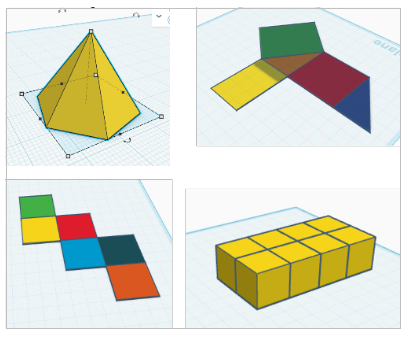
\includegraphics[width=0.4\textwidth]{images/bangun-dan-jaring.png}
            \caption{Desain 3D Bangun Ruang dan Jaring-jaring}
            \label{fig:bangundanjaring}
        \end{figure}
        \item Membuat Gambar Bangun Ruang dengan GeoGebra \\
        \hspace*{1cm}Gambar atau objek matematika yang terdapat dalam media ini sepenuhnya dibuat secara mandiri oleh peneliti. Objek-objek matematika, seperti persegi, kubus, balok, jaring-jaring, serta soal-soal, dibuat menggunakan aplikasi GeoGebra. Berikut ditampilkan contoh hasil pembuatannya.
        \begin{figure}[H]
            \centering
            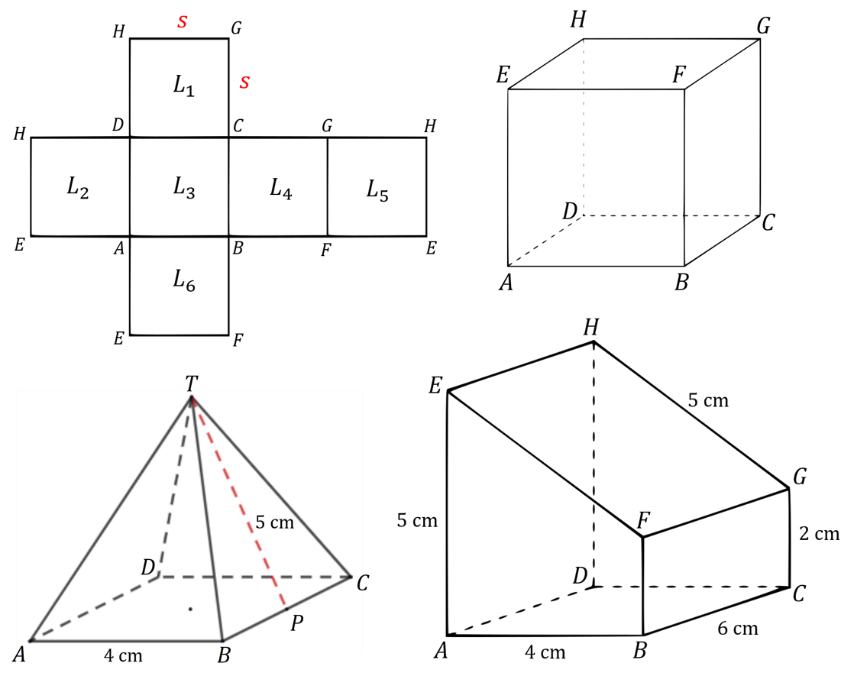
\includegraphics[width=0.4\textwidth]{images/hasil-geogebra.png}
            \caption{Desain 2D Bangun Ruang dan Jaring-jaring}
            \label{fig:hasilgeogebra}
        \end{figure}
        
        \item Membuat UI dengan React JS \\
        \hspace*{1cm}Agar media pembelajaran mudah diakses oleh peserta didik, peneliti membuat antarmuka menggunakan React JS. Antarmuka ini berbentuk situs web, sehingga peserta didik dapat dengan mudah mengakses media melalui domain yang diberikan. Untuk menampilkan simulasi 3D dan Augmented Reality di situs web, peneliti menggunakan Three.js sebagai paket tambahan serta mywebar.com untuk menampilkan konten AR. Berikut ditampilkan contoh hasil pembuatannya.
        \begin{figure}[H]
            \centering
            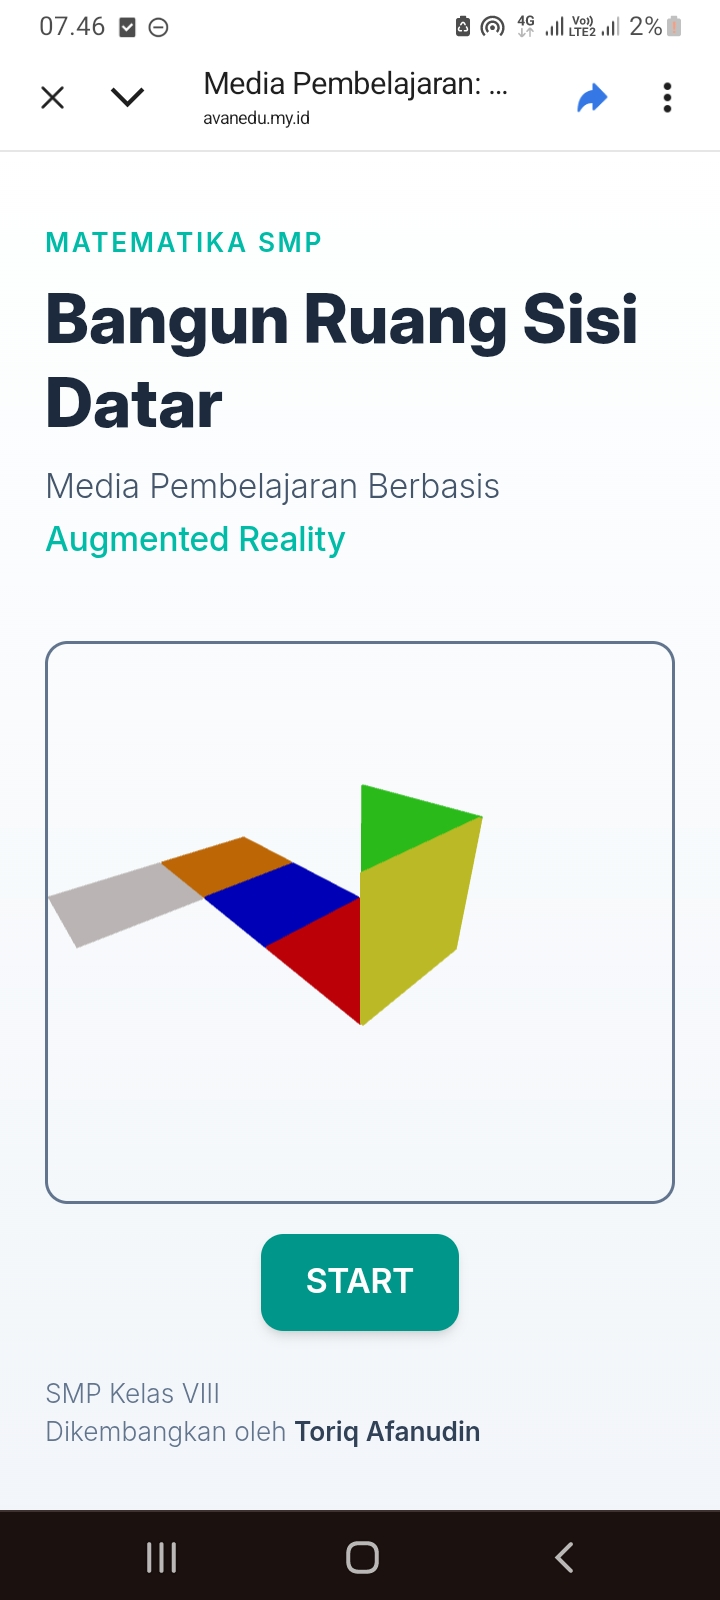
\includegraphics[width=0.3\textwidth]{images/ui-1.jpg}
            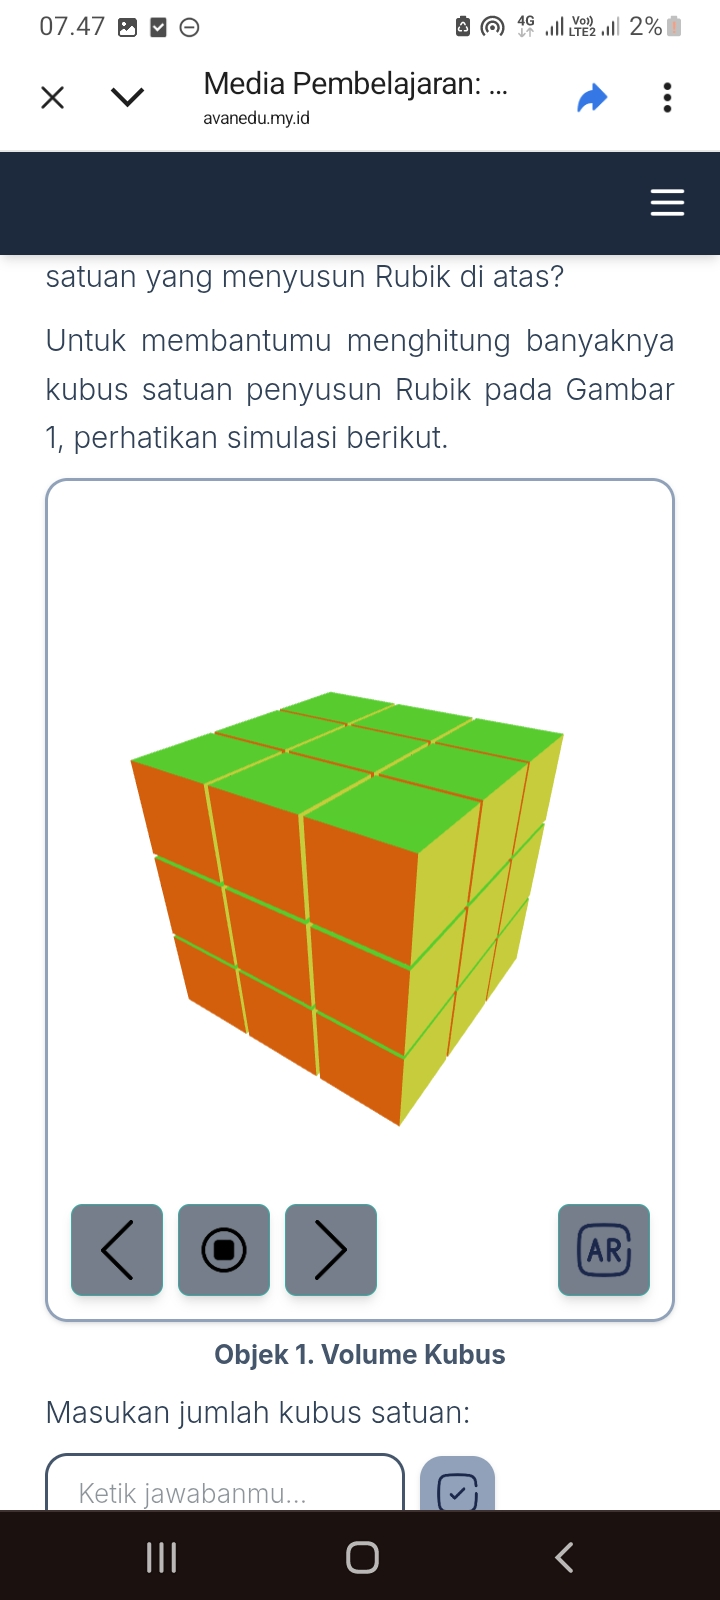
\includegraphics[width=0.3\textwidth]{images/ui-2.jpg}
            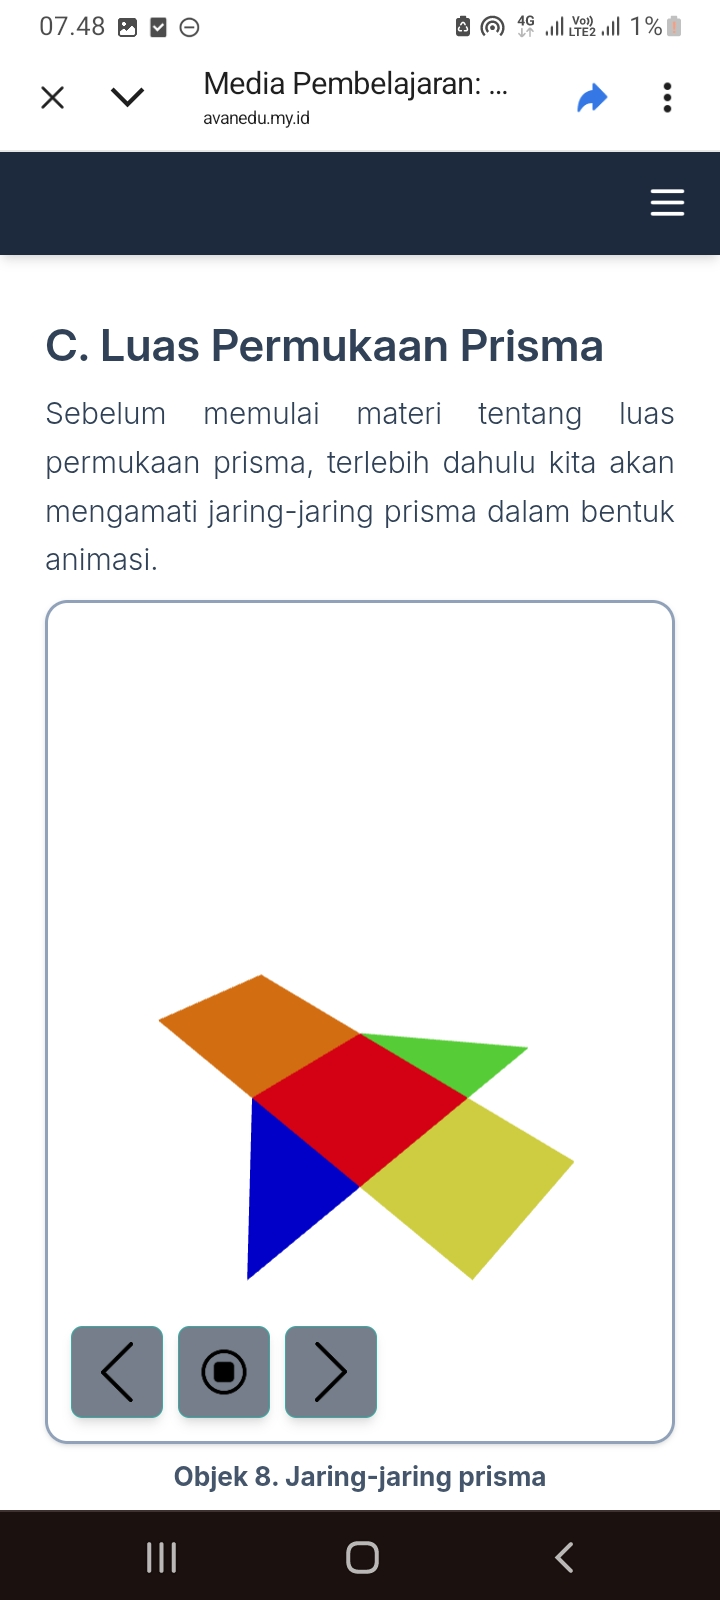
\includegraphics[width=0.3\textwidth]{images/ui-3.jpg}
            \caption{Antarmuka Media AR}
            \label{fig:antarmuka}
        \end{figure}

    \end{enumerate}

    \item \textbf{Implementasi}\\
    \hspace*{1cm}Pada tahap implementasi ini, peneliti melakukan uji coba terhadap produk yang telah dikembangkan. Uji coba dilakukan terhadap peserta didik kelas VIII-D SMP Negeri 3 Kalikajar. Tahap ini bertujuan untuk memperoleh informasi mengenai kelayakan media pembelajaran yang telah dikembangkan. Pada tahap ini, terdapat dua jenis uji coba yang dilakukan, yaitu uji coba kelas kecil dan uji coba kelas besar. Berikut adalah penjelasan mengenai uji coba kelas kecil dan uji coba kelas besar.
    \begin{enumerate}
        \item Uji Coba Kelas Kecil \\
        \hspace*{1cm}Uji coba kelas kecil dilakukan dengan melibatkan beberapa peserta didik dari kelas VIII-D. Pelaksanaan uji coba ini dilakukan melalui kegiatan pembelajaran menggunakan media pembelajaran yang sedang dikembangkan. Setelah pembelajaran selesai, peserta didik diminta mengisi angket untuk memperoleh informasi mengenai respons mereka terhadap media tersebut. Uji coba kelas kecil dilaksanakan pada tanggal 14 Mei 2024 dengan melibatkan 7 peserta didik kelas VIII-D yang dipilih secara acak.

        \hspace*{1cm}Pada tahap awal uji coba kelas kecil, peneliti terlebih dahulu meminta izin kepada pendidik matematika untuk melaksanakan uji coba terhadap 7 peserta didik kelas VIII-D. Pemilihan peserta didik dilakukan secara acak oleh pendidik matematika kelas VIII-D. Uji coba dilakukan dengan memberikan media pembelajaran dan angket kepada peserta didik. Angket tersebut digunakan untuk memperoleh data penilaian peserta didik terhadap media pembelajaran yang sedang dikembangkan. Hasil dari penyebaran angket dapat dilihat pada Tabel 3.

        \item Uji Coba Kelas Besar \\
        \hspace*{1cm}Uji coba kelas besar dilakukan dengan melibatkan seluruh peserta didik kelas VIII-D SMP Negeri 3 Kalikajar pada tanggal 16 Mei 2024. Pemilihan kelas tersebut didasarkan pada rekomendasi dari pendidik matematika. Alasan pemilihan ini adalah karena pendidik mengampu kelas tersebut dan peserta didik diketahui mengalami kesulitan dalam mempelajari materi bangun ruang.

        \hspace{1cm}Uji coba dilakukan melalui pembelajaran menggunakan media pembelajaran berbasis augmented reality. Setelah pembelajaran selesai, peserta didik diberikan angket. Angket tersebut digunakan untuk mengetahui penilaian peserta didik terhadap kualitas media pembelajaran yang dikembangkan. Pembelajaran dilaksanakan dengan membagi peserta didik ke dalam kelompok, disesuaikan dengan jumlah peserta didik yang membawa smartphone. Setelah peserta didik menyelesaikan materi dan soal-soal yang terdapat dalam media, mereka diminta untuk mengisi angket yang telah disediakan.
    \end{enumerate}

    \item \textbf{Evaluasi}
    
    \hspace{1cm}Tahap evaluasi merupakan tahap akhir dalam model pengembangan ADDIE. Evaluasi dilakukan untuk menganalisis hasil uji coba terhadap media pembelajaran berbasis augmented reality pada materi bangun ruang sisi datar kelas VIII. Tujuan dari tahap ini adalah untuk menyempurnakan produk yang telah dikembangkan sebelum menghasilkan produk akhir yang layak digunakan. Selanjutnya, dilakukan revisi akhir berdasarkan masukan dari ahli materi, ahli media, dan peserta didik.

    \hspace{1cm}Berdasarkan hasil validasi dari ahli materi dan ahli media, terdapat beberapa masukan terhadap media pembelajaran yang dikembangkan sebelum dilakukan uji coba kepada peserta didik. Selanjutnya, dilakukan revisi berdasarkan masukan tersebut hingga media pembelajaran masuk dalam kategori baik atau dinyatakan layak. Evaluasi yang dilakukan mencakup hasil validasi dari ahli materi dan ahli media, serta angket hasil uji coba media oleh peserta didik. Penilaian tersebut dijadikan acuan dalam menentukan kelayakan media pembelajaran yang dikembangkan.

\end{enumerate}
% ANALISIS DATA
\textbf{B. Analisis Data}

\hspace{1cm}Analisis data merupakan tahap lanjutan dari tahap evaluasi dalam model pengembangan ADDIE. Data yang diperoleh dalam penelitian ini berupa data kualitatif yang kemudian dikonversi menjadi data kuantitatif. Analisis data dilakukan berdasarkan lembar penilaian dari ahli materi, ahli media, dan respons peserta didik. Media pembelajaran yang dikembangkan dinyatakan layak apabila memperoleh skor rata-rata penilaian dari ahli materi, ahli media, dan respons peserta didik minimal pada kategori “baik”. Berikut ini adalah hasil analisis data tersebut:
\begin{enumerate}
    \item Analisis Penilaian Angket Ahli Materi\\
    \hspace*{1cm}Validasi oleh ahli materi dilakukan untuk memperoleh penilaian berupa skor, komentar, dan masukan terhadap materi yang telah dikembangkan dalam media pembelajaran berbasis augmented reality. Komentar dan saran dari validator digunakan untuk menyempurnakan media pembelajaran agar menghasilkan produk akhir yang layak digunakan. Kelayakan materi dalam media pembelajaran ini dinilai oleh dua orang ahli, yaitu Bapak Aan Hendroanto, M.Sc., dosen Pendidikan Matematika UAD, dan Ibu Wiwik Indarwati, S.Pd., pendidik Matematika di SMP Negeri 3 Kalikajar. Hasil penilaian kelayakan media pembelajaran disajikan pada Tabel \ref{penilaianmateri}.
    \begin{table}[H]
        \begin{adjustwidth}{-2cm}{-2cm}
            \centering
            \caption{Hasil Penilaian Media Pembelajaran Menurut Ahli Media}
            \label{penilaianmateri}
            \begin{tabular}{|c|c|c|c|c|c|}
                \hline
                \textbf{No} & \textbf{Validator} & \textbf{Skor} & \textbf{Rata-rata Skor} & \textbf{Kriteria Data Kuantitatif}\\
                \hline
                1 & Aan Hendroanto, M.Sc. & 0 & 0 & Sangat Baik\\
                2 & Wiwik Indarwati, S.Pd. & 0 & 0 & Sangat Baik\\
                \hline
                \multicolumn{2}{|c|}{Jumlah Skor} & 0 & & \\
                \hline
                \multicolumn{2}{|c|}{Rata-rata Keseluruhan} & 0 & 0 & Sangat Baik\\
                \hline
            \end{tabular}
        \end{adjustwidth}
    \end{table}

    \begin{table}[H]
        \centering
        \caption{Kriteria Penilaian Ahli Materi}
        \begin{tabular}{|c|c|c|}
            \hline
            \textbf{No} & \textbf{Rentang Skor \( (i) \) Kuantitatif} & \textbf{Kategori Kualitatif}\\
            \hline
            1 & \( \bar{x} > 4{,}21 \) & Sangat Baik\\
            2 & \( 3{,}41 < \bar{x} \leq 4{,}2 \) & Baik\\
            3 & \( 2{,}60 < \bar{x} \leq 3{,}41 \) & Cukup Baik\\
            4 & \( 1{,}80 < \bar{x} \leq 2{,}60 \) & Kurang\\
            5 & \( \bar{x} \leq 1{,80} \) & Sangat Kurang\\
            \hline 
        \end{tabular}
    \end{table}

    \item Analisis Penilaian Angket Ahli Media\\
    \hspace*{1cm}Validasi oleh ahli media dilakukan untuk memperoleh penilaian berupa skor, komentar, dan masukan terhadap media pembelajaran yang dikembangkan. Komentar dan saran dari validator media digunakan untuk menyempurnakan media pembelajaran agar menghasilkan produk akhir yang layak digunakan. Kelayakan media pembelajaran ini dinilai oleh dua orang ahli media, yaitu Bapak Anggit Prabowo, M.Pd., dosen Pendidikan Matematika UAD, dan Ibu Wiwik Indarwati, S.Pd., pendidik Matematika di SMP Negeri 3 Kalikajar. Hasil penilaian kelayakan oleh ahli media disajikan pada Tabel~\ref{penilaianmedia}.
    \begin{table}[H]
        \begin{adjustwidth}{-2cm}{-2cm}
            \centering
            \caption{Hasil Penilaian Media Pembelajaran Menurut Ahli Media}
            \label{penilaianmedia}
            \begin{tabular}{|c|c|c|c|c|c|}
                \hline
                \textbf{No} & \textbf{Validator} & \textbf{Skor} & \textbf{Rata-rata Skor} & \textbf{Kriteria Data Kuantitatif}\\
                \hline
                1 & Anggit Prabowo, M.Pd. & 150 & \( 4{,}41 \) & Sangat Baik\\
                2 & Wiwik Indarwati, S.Pd. & 0 & 0 & Sangat Baik\\
                \hline
                \multicolumn{2}{|c|}{Jumlah Skor} & 0 & & \\
                \hline
                \multicolumn{2}{|c|}{Rata-rata Keseluruhan} & 0 & 0 & Sangat Baik\\
                \hline
            \end{tabular}
        \end{adjustwidth}
    \end{table}

    \begin{table}[H]
        \centering
        \caption{Kriteria Penilaian Ahli Media}
        \begin{tabular}{|c|c|c|}
            \hline
            \textbf{No} & \textbf{Rentang Skor \( (i) \) Kuantitatif} & \textbf{Kategori Kualitatif}\\
            \hline
            1 & \( \bar{x} > 4{,}21 \) & Sangat Baik\\
            2 & \( 3{,}41 < \bar{x} \leq 4{,}2 \) & Baik\\
            3 & \( 2{,}60 < \bar{x} \leq 3{,}41 \) & Cukup Baik\\
            4 & \( 1{,}80 < \bar{x} \leq 2{,}60 \) & Kurang\\
            5 & \( \bar{x} \leq 1{,80} \) & Sangat Kurang\\
            \hline 
        \end{tabular}
    \end{table}

    \item Analisis Penilaian Angket Respons Peserta Didik\\
    \hspace*{1cm}Respons peserta didik diperoleh melalui uji coba kelas kecil dan uji coba kelas besar yang bertujuan untuk mendapatkan penilaian berupa skor, komentar, dan masukan terhadap media pembelajaran yang telah dikembangkan. Respons tersebut dianalisis berdasarkan hasil angket yang disebarkan kepada peserta didik kelas VIII-D SMP Negeri 3 Kalikajar. Kriteria penilaian angket respons peserta didik disajikan pada Tabel \ref{kriteriaresponsiswa}.
    \begin{table}[H]
        \centering
        \caption{Kriteria Penilaian Respon Peserta Didik}
        \label{kriteriaresponsiswa}
        \begin{tabular}{|c|c|c|}
            \hline
            \textbf{No} & \textbf{Rentang Skor \( (i) \) Kuantitatif} & \textbf{Kategori Kualitatif}\\
            \hline
            1 & \( \bar{x} > 4{,}21 \) & Sangat Baik\\
            2 & \( 3{,}41 < \bar{x} \leq 4{,}2 \) & Baik\\
            3 & \( 2{,}60 < \bar{x} \leq 3{,}41 \) & Cukup Baik\\
            4 & \( 1{,}80 < \bar{x} \leq 2{,}60 \) & Kurang\\
            5 & \( \bar{x} \leq 1{,80} \) & Sangat Kurang\\
            \hline 
        \end{tabular}
    \end{table}
    \item Kualitas Produk Secara Keseluruhan\\
    \hspace*{1cm}Kualitas media pembelajaran secara keseluruhan dinilai berdasarkan skor rata-rata dari ahli materi, ahli media, uji coba kelas kecil, dan uji coba kelas besar. Hasil perhitungan rata-rata keseluruhan dari keempat penilaian tersebut disajikan pada Tabel~\ref{ratakeseluruhan}.\\
    \begin{table}[H]
        \centering
        \caption{Hasil Rata-rata Keseluruhan}
        \label{ratakeseluruhan}
        \begin{tabular}{|c|c|c|c|}
            \hline
            \textbf{No} & \textbf{Sampel Uji Coba} & \textbf{Rata-rata} & \textbf{Kriteria}\\
            \hline
            1 & Ahli Materi & 0 & Sangat Baik\\
            2 & Ahli Media & \( 4{,}41 \) & Sangat Baik\\
            3 & Uji Coba Kelas Kecil & 0 & Sangat Baik\\
            4 & Uji Coba Kelas Besar & \( 4{,}19 \) & Baik\\
            \hline
            \multicolumn{2}{|c|}{Rata-rata Keseluruhan} & 0 & Sangat Baik\\
            \hline
            
        \end{tabular}
    \end{table}
    \hspace*{1cm}Berdasarkan Tabel~\ref{ratakeseluruhan}, terlihat bahwa hasil perhitungan rata-rata secara keseluruhan dari ahli materi, ahli media, uji coba kelas kecil, dan uji coba kelas besar memperoleh skor rata-rata sebesar XXX dan termasuk dalam kategori sangat baik. Dengan demikian, media pembelajaran berbasis augmented reality yang dikembangkan dinyatakan layak untuk digunakan.

\end{enumerate}
% REVISI PRODUK
\textbf{C. Revisi Produk}

\hspace*{1cm}Revisi produk merupakan langkah penting dalam pengembangan media pembelajaran. Revisi dilakukan apabila masih terdapat kesalahan atau kekurangan pada produk yang dikembangkan. Pada tahap ini, peneliti melakukan revisi terhadap media pembelajaran berdasarkan saran dan masukan dari ahli materi dan ahli media. Adapun proses revisi dalam pengembangan media pembelajaran ini adalah sebagai berikut:
\begin{enumerate}
    \item Revisi Produk Hasil Validasi Ahli Materi\\
    \hspace*{1cm}Berdasarkan masukan dari ahli materi, perbaikan yang dilakukan telah sesuai dengan saran dan rekomendasi yang diberikan. Hasil perbaikan tersebut disajikan sebagai berikut.
    \begin{enumerate}
        \item Menambahkan kelas dan logo UAD pada halaman sampul.
        \item Menambahkan ilustrasi kubus satuan yang tidak dapat dihitung menggunakan tombol.
        \item Menyisipkan teknologi AR pada soal, tidak hanya pada materi.
        \item Menambahkan materi mengenai unsur-unsur bangun ruang.
        \item Memperbaiki penggunaan tanda baca pada kalimat-kalimat dalam media.
    \end{enumerate}
    \item Revisi Produk Hasil Validasi Ahli Media
    \item Revisi Produk Hasil Uji Coba Kelas Kecil
    \item Revisi Produk Hasil Uji Coba Kelas Besar
\end{enumerate}

\textbf{D. Kajian Produk Akhir}

\hspace*{1cm}Media pembelajaran yang dikembangkan oleh peneliti disusun dengan isi sebagai berikut:
\begin{enumerate}
    \item Halaman Sampul\\
    \hspace*{1cm}Halaman ini menampilkan judul, judul materi, sasaran, serta nama pengembang.
    \begin{figure}[H]
        \centering
        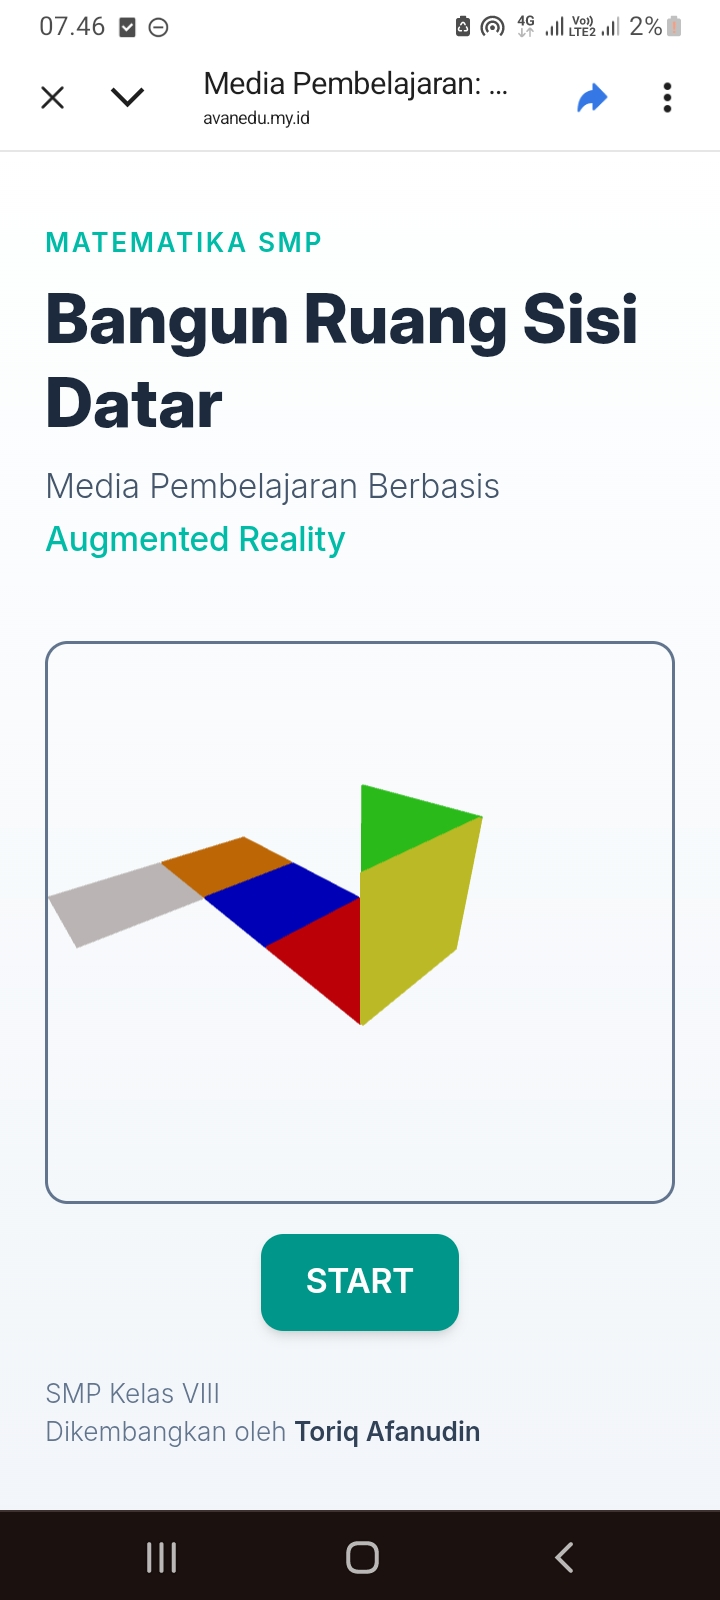
\includegraphics[width=0.3\textwidth]{images/ui-1.jpg}
        \caption{Halaman Sampul}
        \label{fig:sampul}
    \end{figure}
    \item Halaman Petunjuk\\
    \hspace*{1cm}Pada halaman ini, peserta didik dapat mengunduh barcode yang dibutuhkan untuk menampilkan augmented reality (AR) serta berlatih menggunakan AR sebelum memulai pembelajaran.
    \begin{figure}[H]
        \centering
        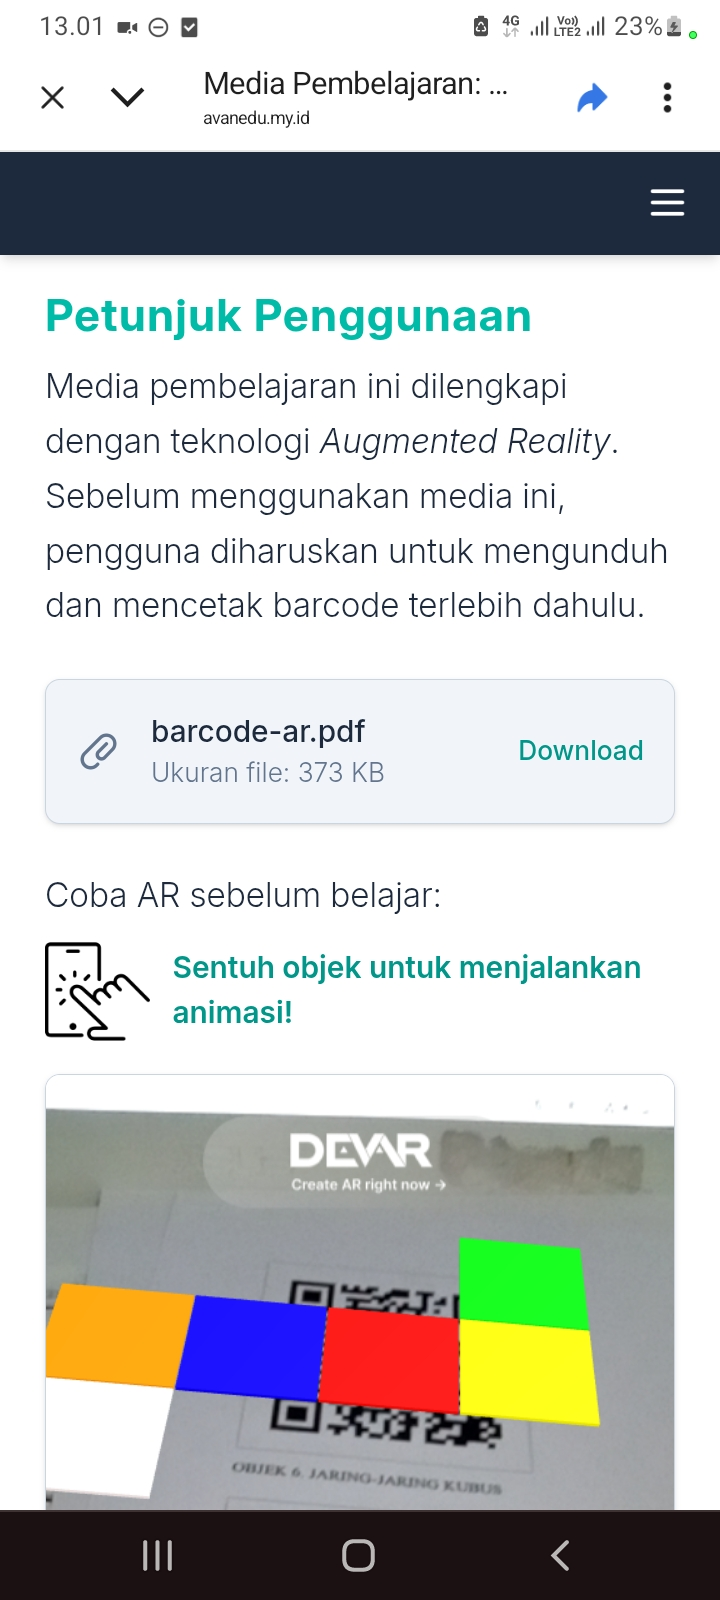
\includegraphics[width=0.25\textwidth]{images/petunjuk.jpg}
        \caption{Halaman Petunjuk}
        \label{fig:petunjuk}
    \end{figure}
    \item Halaman Menu\\
    \hspace*{1cm}Pada halaman ini, peserta didik dapat memilih materi yang ingin dipelajari atau langsung mengerjakan kuis.
    \begin{figure}[H]
        \centering
        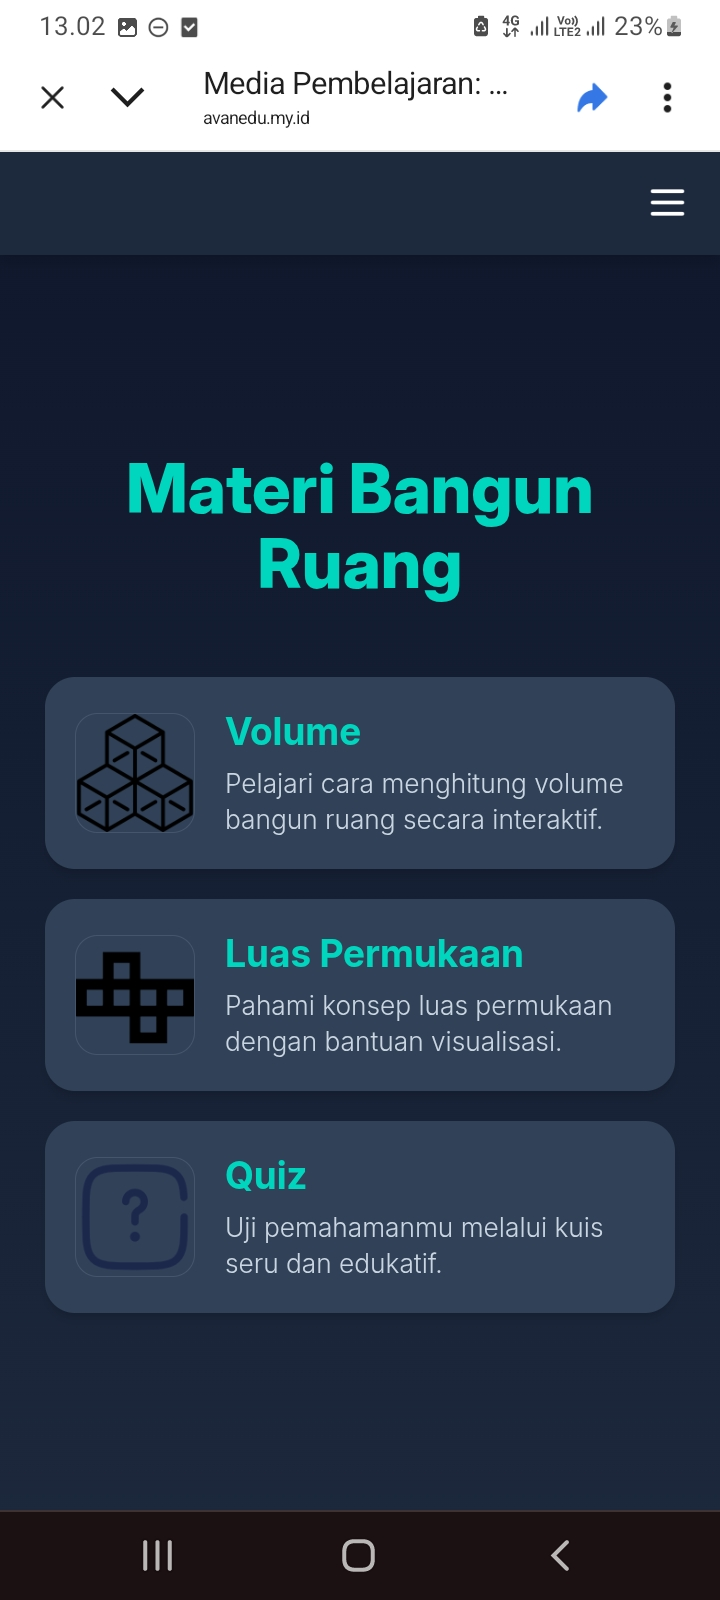
\includegraphics[width=0.2\textwidth]{images/menu.jpg}
        \caption{Halaman Menu}
        \label{fig:menu}
    \end{figure}

    \item Halaman Materi\\
    \hspace*{1cm}Pada halaman materi, peserta didik akan mempelajari dua topik utama, yaitu volume dan luas permukaan bangun ruang. Peserta didik akan melihat bangun ruang yang disajikan dalam bentuk 3D dan augmented reality. Bangun ruang tersebut juga dapat dianimasikan untuk mempermudah pemahaman. Untuk mengevaluasi pemahaman peserta didik, tersedia latihan soal di akhir setiap bab.
    \begin{figure}[H]
        \centering
        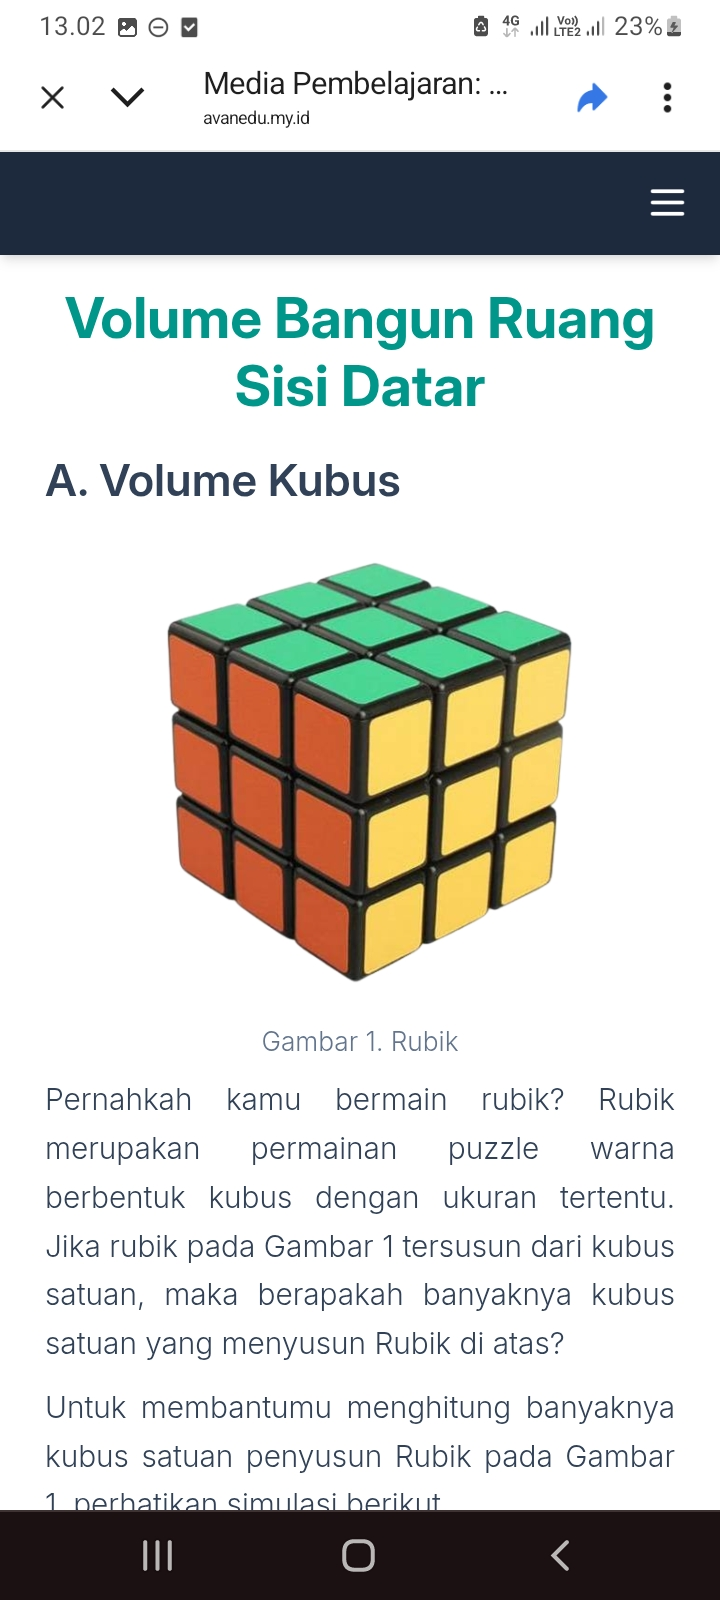
\includegraphics[width=0.2\textwidth]{images/materi1.jpg}
        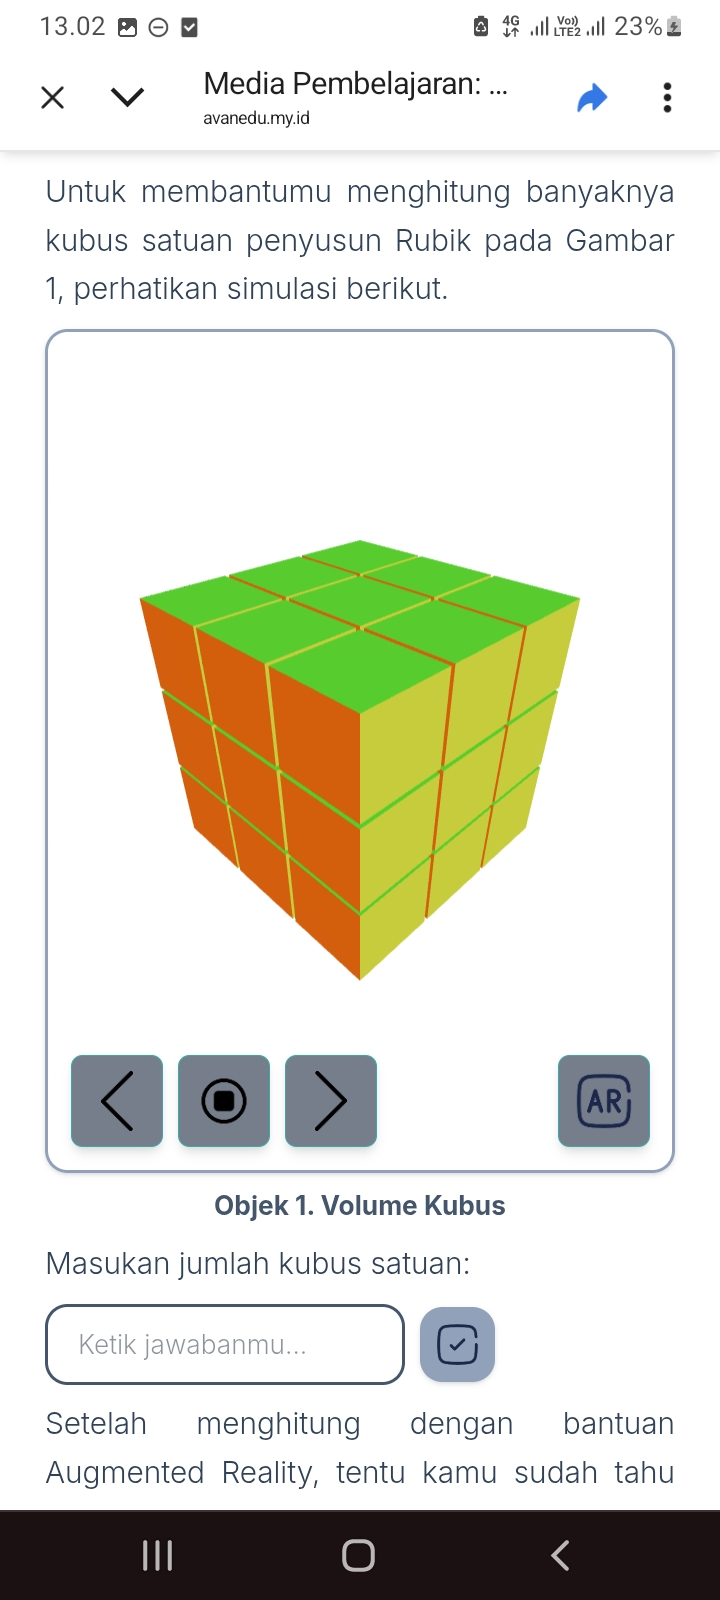
\includegraphics[width=0.2\textwidth]{images/materi2.jpg}
        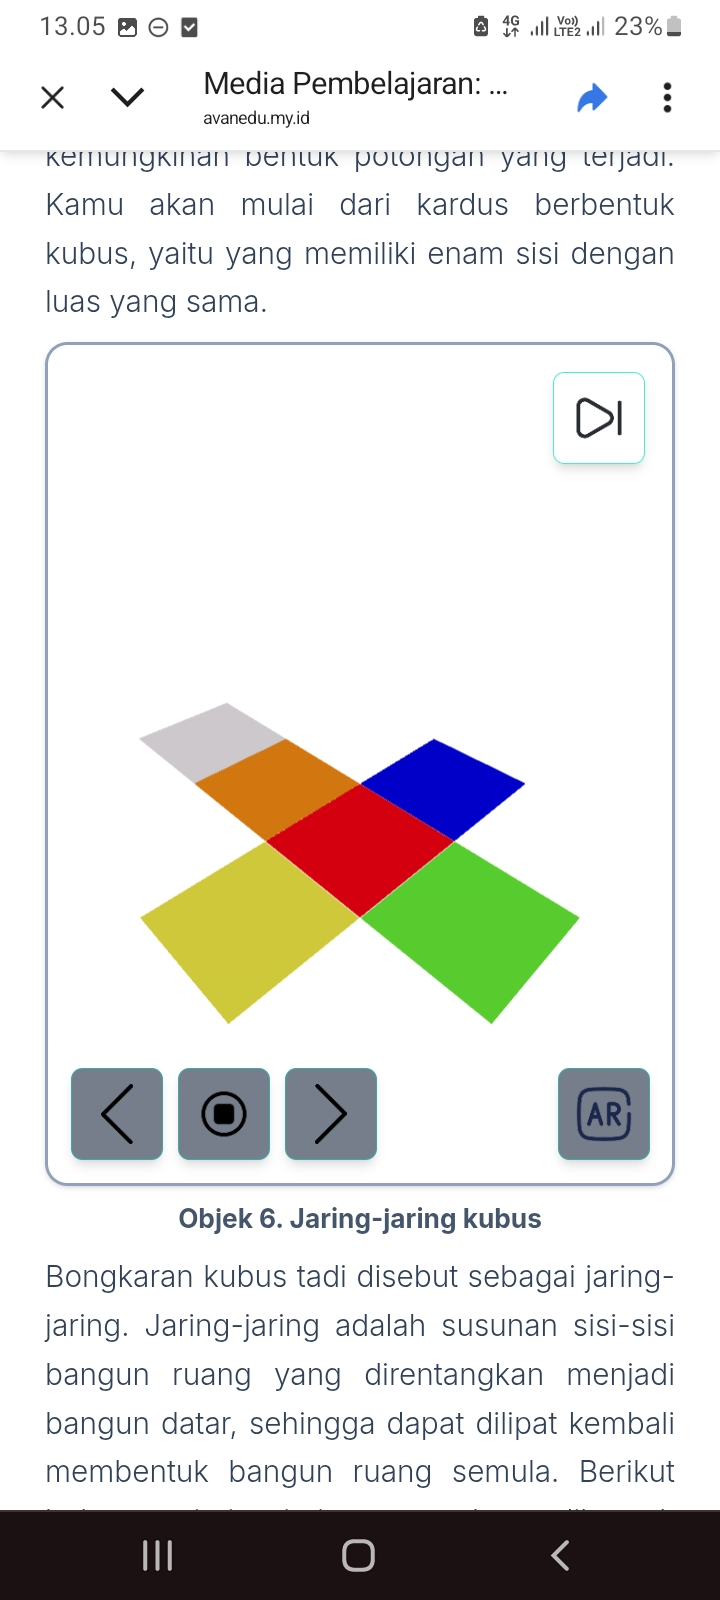
\includegraphics[width=0.2\textwidth]{images/materi3.jpg}
        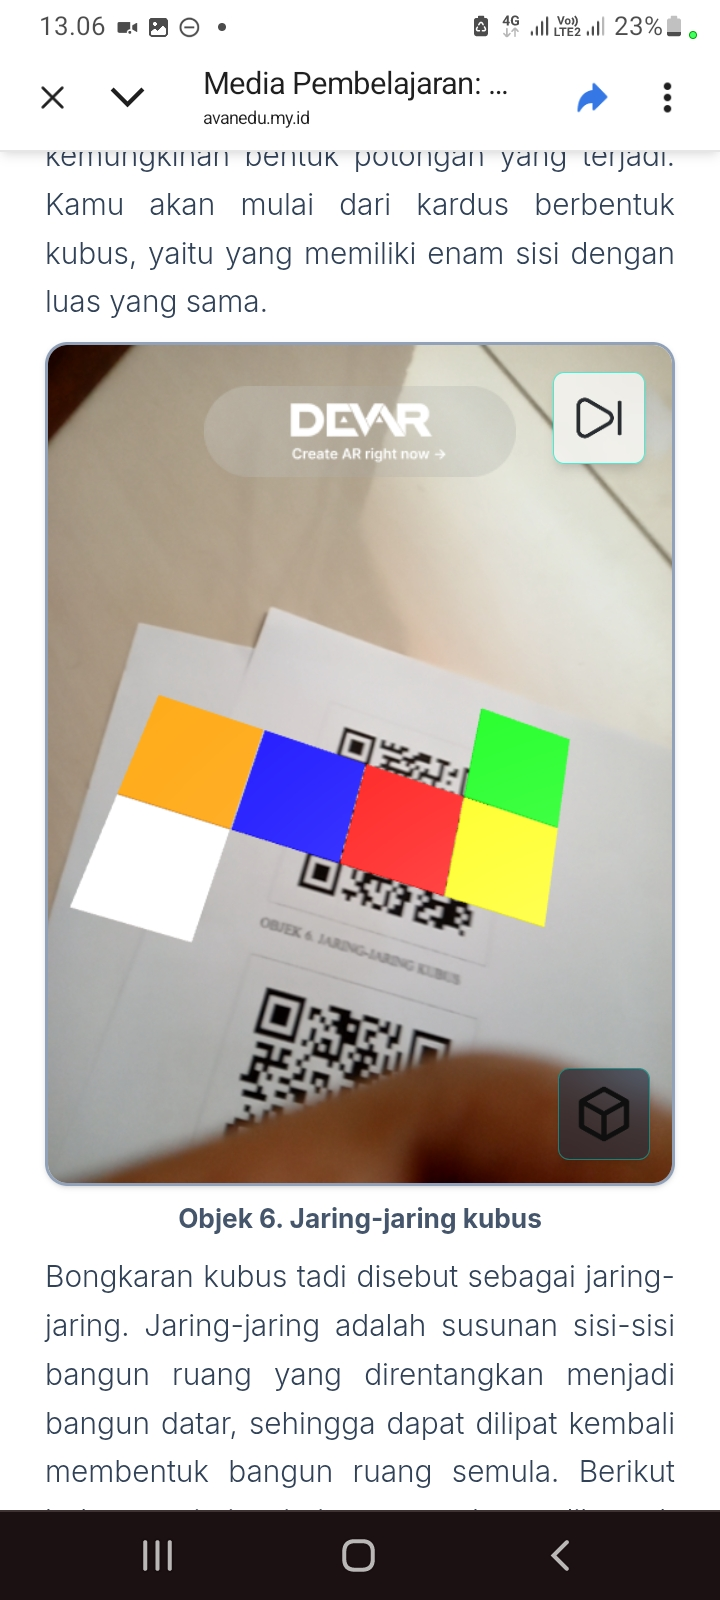
\includegraphics[width=0.2\textwidth]{images/materi4.jpg}
        \caption{Halaman Materi}
        \label{fig:materi}
    \end{figure}

    \item Halaman Kuis\\
    \hspace*{1cm}Pada halaman kuis, disajikan lima soal yang sesuai dengan latihan soal di akhir setiap bab. Terdapat juga penghitung waktu (timer) dengan batas waktu pengerjaan selama 30 menit. Untuk mulai mengerjakan kuis, peserta didik perlu memasukkan kode ujian. Peserta didik dapat menjawab soal dengan mengisi kolom jawaban yang disediakan, serta dapat menyisipkan foto untuk memperkuat jawabannya.
    \begin{figure}[H]
        \centering
        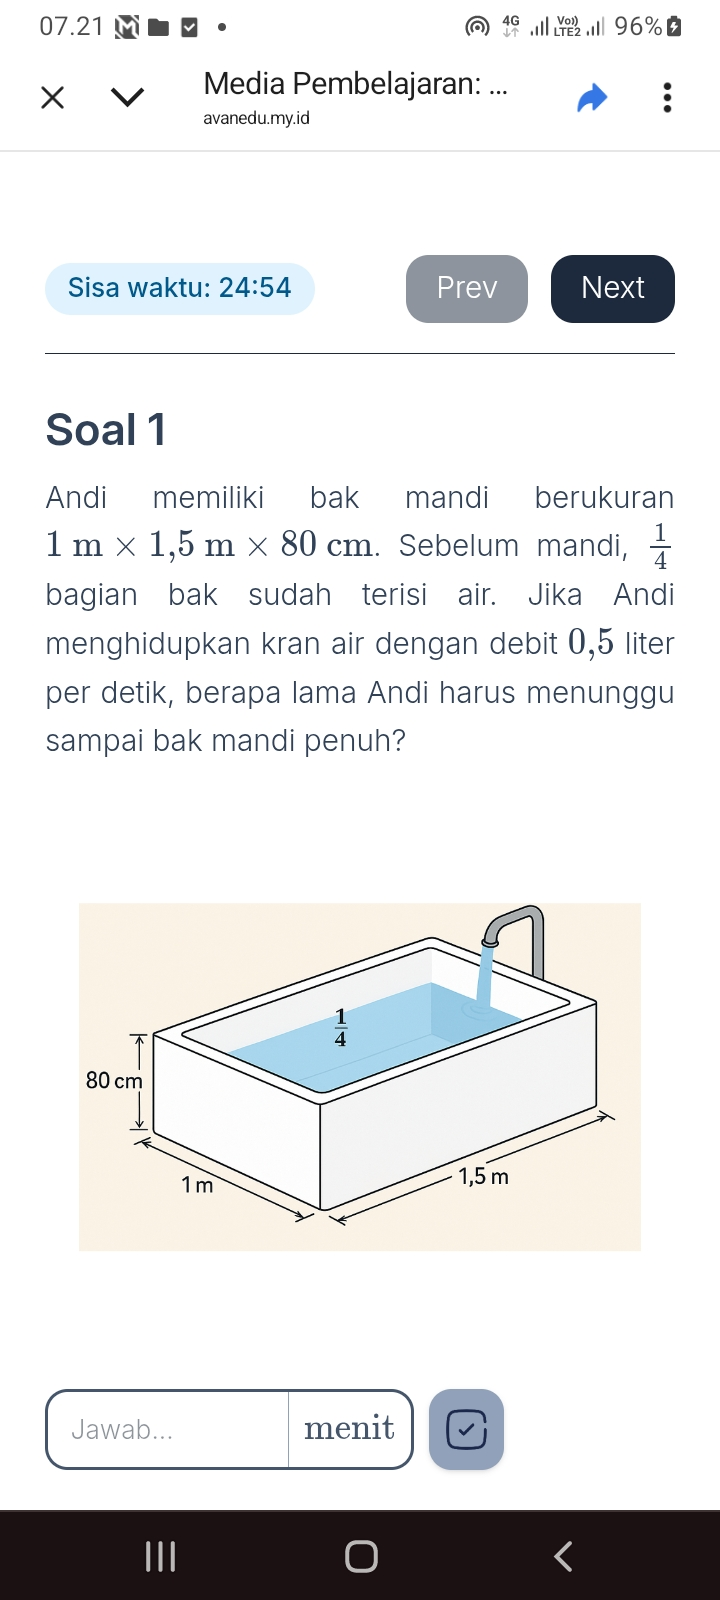
\includegraphics[width=0.25\textwidth]{images/kuis1.jpg}
        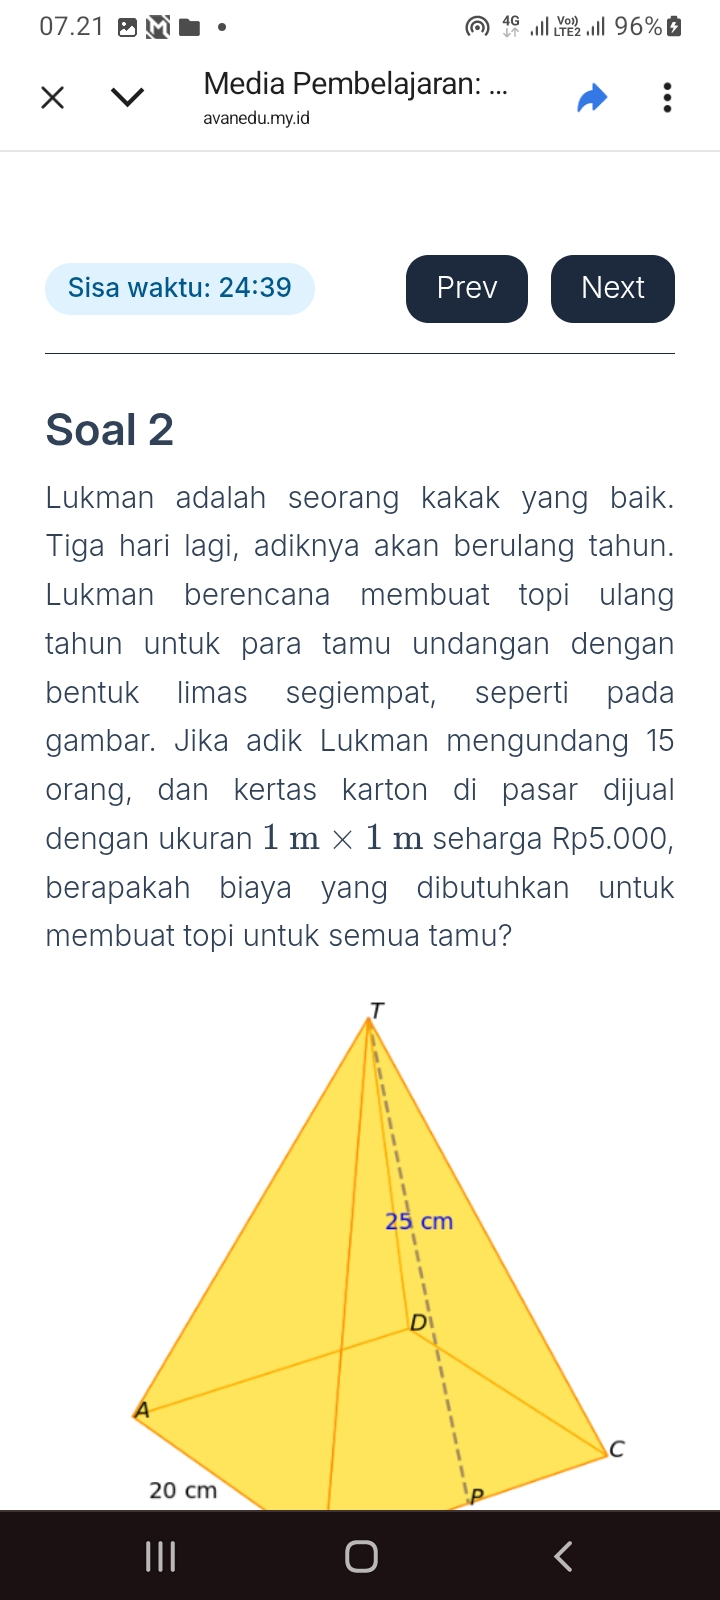
\includegraphics[width=0.25\textwidth]{images/kuis2.jpg}
        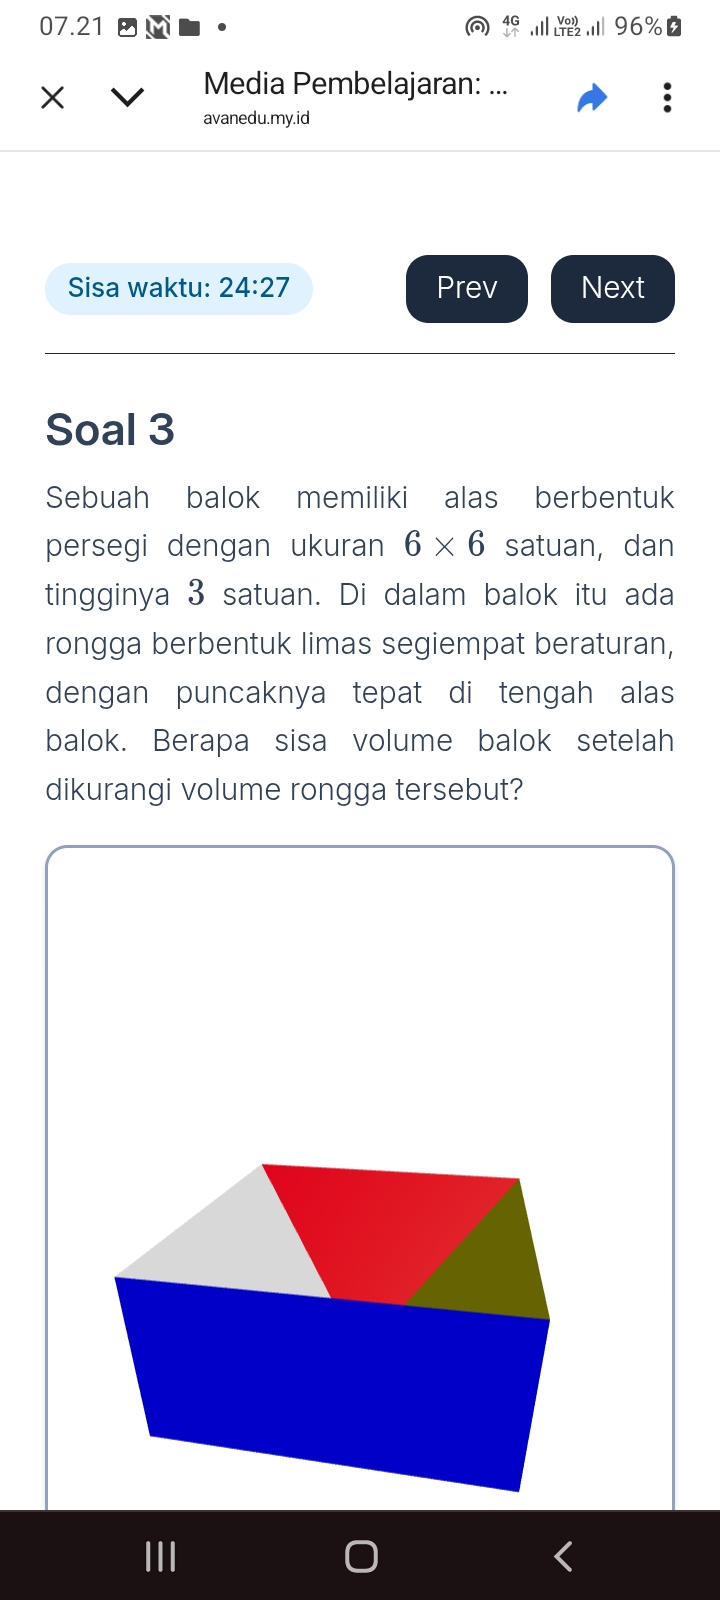
\includegraphics[width=0.25\textwidth]{images/kuis3.jpg}
        \caption{Halaman Kuis}
        \label{fig:kuis}
    \end{figure}

\end{enumerate}
\newpage
\bibliography{daftar-pustaka}


\end{document}
